% Winter regime chapter
\chapter{Downwelling regime}\label{ch:winter}

\section{Introduction}
As we have seen in the previous chapter, a poleward flowing
undercurrent is intrinsic to most upwelling systems
\citep{Neshyba89} and the Galician upwelling system is no
exception. Along-slope variability in wind stress forcing or
topography can be called upon to explain its presence in the face
of upwelling favourable winds \citep{Wang97,Trowbridge98}.
However, the Galician upwelling regime is only present for part of
the year (June-October). The rest of the year, a downwelling
regime with a surface poleward flow settles in the shelf, and in
the absence of upwelling, other forcings drive the slope poleward
flow. Northward winds represent a possible mechanism except, as
shown in chapter~\ref{ch:winds}, they are highly variable. They
more likely contribute to the short temporal variability
associated with the poleward flow while an oceanic pressure
gradient is responsible for its seasonal onset
\citep{Frouin90,Haynes90}. Steady-state adjustment of an
alongshore oceanic pressure gradient adjacent to a steep
continental slope would fail to penetrate the shelf \citep{Wang82}
as described in terms of the arrested topographic wave model of
\citet{Csanady78}. Shelf-ocean adjustment is confined to the slope
region and results in a poleward slope-trapped current on eastern
boundaries \citep{Hill98}. Assuming the oceanic sea-level gradient
is physically due to the meridional drop in steric height arising
from the fall in oceanic temperatures poleward,
\citet{Huthnance84,Huthnance95} described the JEBAR effect ({\it
joint effect of baroclinicity and relief}). Zonally oriented
density surfaces intersect a meridional sloping boundary and a
dynamical adjustment of the density-induced pressure gradient to
the bottom slope takes place. The JEBAR effect should apply along
the entire eastern boundary but is most relevant upstream of
regions where steric height drops markedly. A meridional density
gradient is maximum between 39\deg N and 41\deg N \citep{Arhan94}
but weakens/disappears northwards. At 43\deg N, the slope turns
zonally and the JEBAR mechanism no longer forces the poleward flow
directly. In the absence of direct forcing and considering
frictional effects, \citet{Pingree90} showed that the JEBAR
induced poleward slope flow decays with a length scale smaller
than the northern Spanish coast, and hence propagates along the
slope away from the source reaching the French coast of the Bay of
Biscay. Temporally varying spatial structures in the California
undercurrent have been related to the interaction of the current
with the complex topography \citep{Noble00}, but the relevance of
this in the Galician region remains to be assessed.

\section{Cruise Description}
The data presented in this chapter were largely collected during
13 October-7 November 1999 cruise on board the R/V Thalassa in the
Galician region. The cruise was divided into two legs with
different objectives. The aim for Leg A (13-20 October) was to
sample OMEXII-II S, P, and N reference transects (see
chapter~\ref{ch:spring}, Fig.~\ref{fig:cd105stations} for
location) during the autumn and study the distribution of
physical, biological and chemical properties. This was to enable
the building of biogeochemical budgets for input to models of the
exchange of material between the continental shelf and the ocean
at seasonal scales. Leg B (20 October-7 November) had as a main
objective to study the physical structure and biological
functioning of a Slope Water Oceanic eDDY (SWODDY) previously
identified in SST images. Bad weather and lack of evidence in the
hydrography of such structures influenced the decision to continue
sampling the poleward flow seen during Leg A at more northern
latitudes, hence providing one of the most detailed samplings of
the poleward flow around the Galician coast. Nearshore transects
and CTD stations occupied during the entire cruise can be seen in
Fig.~\ref{fig:thal_adcp_st}.

\begin{figure}
\centering \arribacap
\subfigure[]{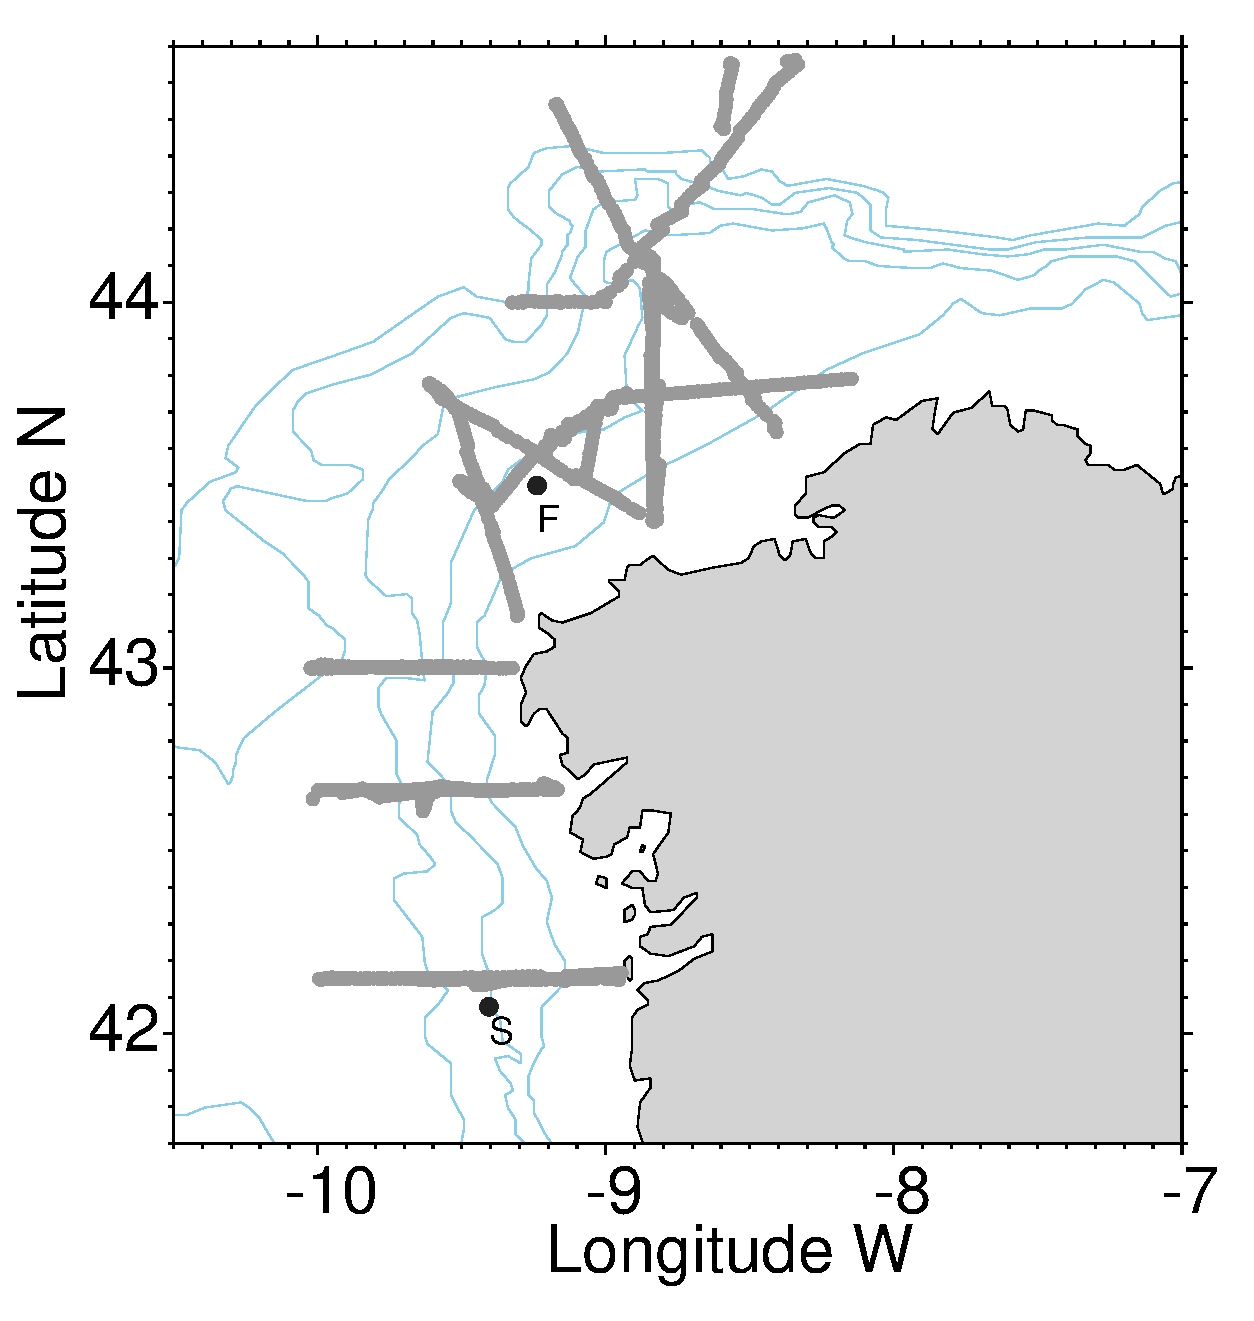
\includegraphics[width=7cm]{stations}}
\subfigure[]{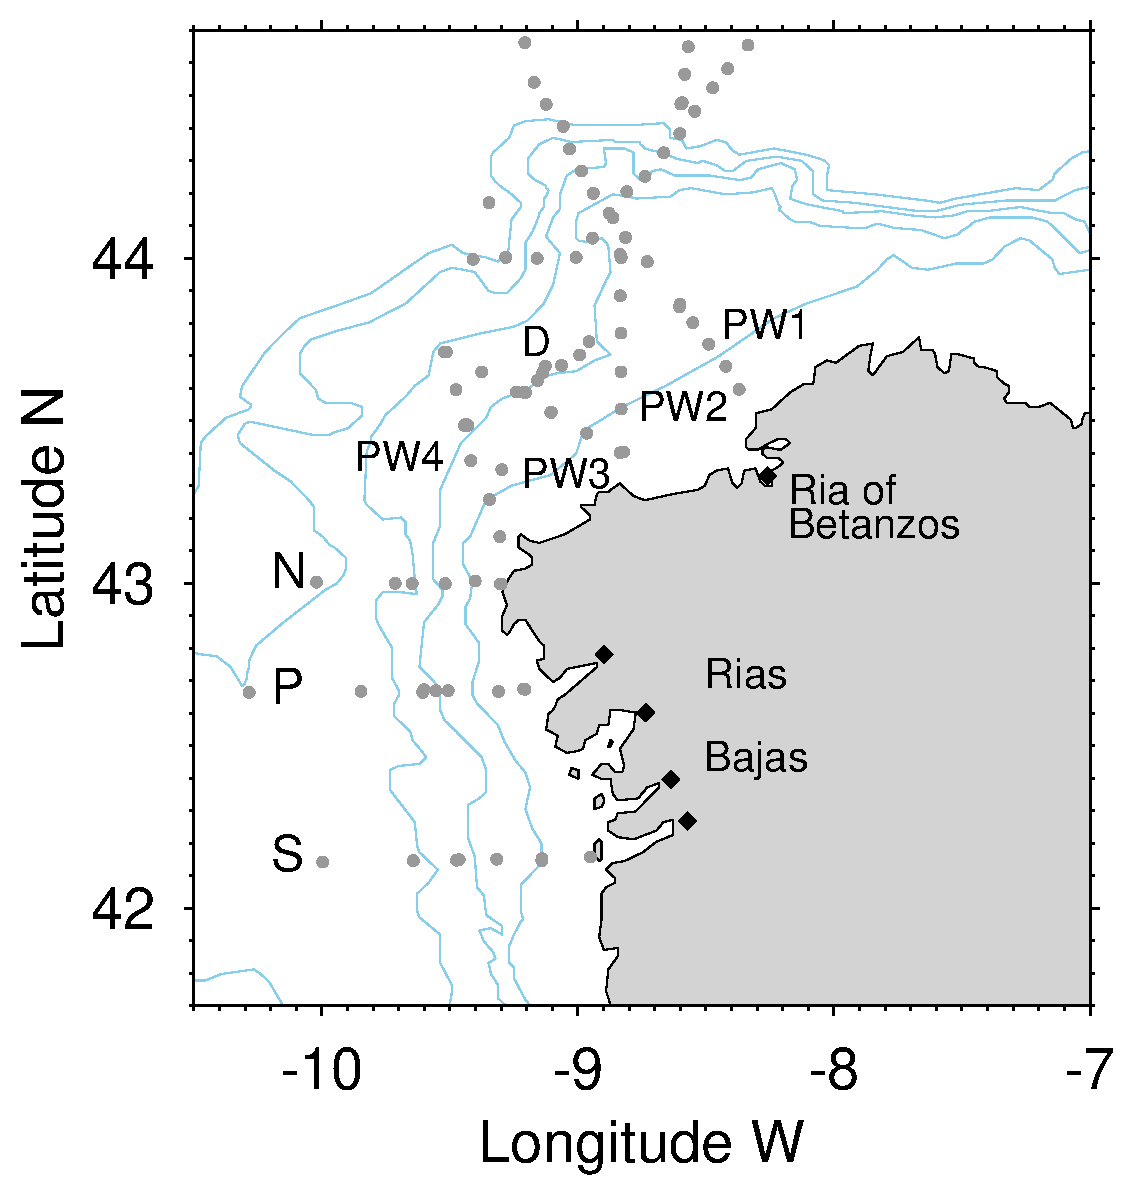
\includegraphics[width=7cm]{ctdstations}} \caption{
ADCP transects and CTD stations positions visited during the
THAL99 cruise (13 October-7 November 1999). Black diamonds mark
the fresh water sources along the Galician coast. Buoys S and F
are also labelled.} \label{fig:thal_adcp_st}
\end{figure}

\section{Data and methods}
A total of 120 CTD drops was made with a 24-position Rossette
(General Oceanics) sampler coupled to a Neil Brown Systems Mk IIIB
CTD with temperature, conductivity, pressure and fluorescence
sensors. Pre-cruise calibration of the temperature sensor
undertaken by the Unidad Tecnologica Marina (previously Unidad de
Gestion de Buques Oceanograficos e Instalaciones Polares) from
Barcelona showed it was working to the manufacturer's
specifications. The conductivity sensor was calibrated against 42
bottle samples collected during the cruise, encompassing the whole
depth range of measurements, with a Guildline Autosal\circledR \,
salinometer giving the calibration equation,
\begin{equation}
S_c=0.921\times S_u (\pm 0.03) + 2.81 (\pm 1.3)
\end{equation}
with correlation $r^2=0.956$, where $S_c$ stands for corrected
salinity and $S_u$ for uncorrected salinity. Associated errors at
95\% confidence are enclosed in brackets. Casts were made to a
specified depth of 500m or the sea bottom if shallower. For
information on the Biological and Chemical measurements see
\citet{Varelaomex00,Varela00}. On several occasions, transects of
the top 100m were sampled with a towed undulating CTD, the
Aquashuttle Undulating Oceanographic Recorder (UOR) from Chelsea
Instruments. The UOR is a multisensor instrument measuring
underway conductivity, temperature, pressure, fluorescence and
photosynthetically active irradiance (PAR). The depth range
sampled depends on the towing speed and the length of the cable.
The typical depth range during the cruise was 30-100m at a towing
speed of 8kt.

Underway measurements of temperature, salinity and fluorescence
were taken every 10min with a SeaBird 21 Thermosalinometer from
the continuous water supply from a nominal depth of 5m.
Meteorological data were measured with a Vaisala MILOS 500 weather
unit and recorded every 10min together with the navigational data.

The Thalassa R/V is equipped with two RDI ADCP that were used
simultaneously during the cruise. Both the 150Khz broadband (BB)
and 75Khz narrowband (NB) performed relatively well in spite of
the bad weather conditions encountered during the cruise. The
systems were running on two different PC with RDI Transect
software. The 150Khz BB ADCP, firmware 5.52, is a four beam
transducer, with a beam angle of 20\deg and a concave
configuration. The 75Khz NB ADCP, firmware 1712, had the same
configuration, and both presented a misalignment angle of 45\deg
which was accounted for in the software settings. The systems were
installed at 6m depth.

The two systems differ not only in their operating frequency but
in the way they measure water velocities. Narrowband ADPCs measure
frequency shifts of single sound pulses and transform it into
velocity estimates through the Doppler Effect. Broadband ADCPs
instead measure the phase shift of multiple echoes, i.e. over a
broad range of frequencies, taking advantage of the full signal
bandwidth available for measuring velocity. Each broadband sound
pulse contains many shorter coded pulses and the final velocity
value is the average of multiple estimates. The phase ambiguity
associated with this technique is resolved by autocorrelation
methods. Broadband Doppler phase processing is equivalent
mathematically to using the Doppler shift of frequency but employs
a method for estimating velocity that results in better accuracy
than with narrowband ADCP.

There is an inverse relationship between sound absorption and
frequency which translates into a greater penetration of the 75Khz
system compare to the 150Khz. The difference is further increased
because the BB system has a reduced depth penetration at an
equivalent working frequency in favour of greater accuracy in
shorter averaging intervals. A summary of the configuration used
in the two systems is given in Table~\ref{tb:thaladcpcon}.

\begin{table}[ht]
  \centering
\begin{tabular}{cccccccc}
\hline \hline \multicolumn{7}{c}{Characteristics of ADCP system setup}\\
\cline{1-8}
 & Cell  & Pulse  & Blanking  & No of  &
Pings per  & Averaging  & Pitch \& roll  \\
 & length & length  &  interval &  bins &
 ensemble &  interval &  compensation \\
\cline{1-8}
75Khz&16m&16m&16m&50&4&300s&No\\
150Khz&8m&8m&8m&50&1&300s&No\\
\hline \hline
\end{tabular}
  \caption{Configuration setup for cruise Thal99}\label{tb:thaladcpcon}
\end{table}

The processing of both datasets followed the technique described
in Chapter~\ref{ch:spring} and only a brief assessment of the data
quality will be presented. The percentage of good bins processed
by both ADCPs (Fig.~\ref{fig:winterpgood}) was high during most of
the cruise ($>$80\%) except at times of rough weather. Typical
depth penetration was 500m for the NB ADCP and 200m for the BB
ADCP, on occasions reaching 600m and 250m respectively. The BB
ADCP showed worse data quality at times when the ship was sailing
against the predominant sea (Fig.~\ref{fig:winterpgood}, days
306.5 and 307.5) as it was fixed closer to the prow with respect
to the NB ADCP. The shallower bins do not seem to be contaminated
as was the case with the R/V Charles Darwin cruises, an indication
that the problem was caused by a less than optimal installation in
the R/V Charles Darwin.

The calibration of both systems was done as described in
section~\ref{sec:springcal} using the water track method.
Estimation of the amplitude and phase was done by averaging 190
and 182 points for the NB and BB ADCP respectively. Mean and
standard deviation values are shown in Table~\ref{tb:wintercal}.
The largest associated uncertainties in the calibration parameters
come from the standard deviation of the phase misalignment angle
which could introduce spurious speeds of up to 7\velc\, at a
highest ship speed of $\sim$5\vel.

\begin{table}[th]
  \centering
\begin{tabular}{cllll}
\hline \hline & \multicolumn{2}{c}{$\beta \, \pm \, \sigma$} &
\multicolumn{2}{c}{$\alpha \, \pm \, \sigma$} \\ \cline{1-5}
75 Khz & 0.98 & $\pm 0.01$ & 0.2 & $\pm 0.8 $\\
150 Khz & 0.99 & $\pm 0.01$ & 0.9 & $\pm 0.8 $\\
\hline \hline
\end{tabular}
  \caption{Calibration parameters for THAL99}\label{tb:wintercal}
\end{table}
\begin{figure}
\hspace*{2.8cm}\subfigure[]{
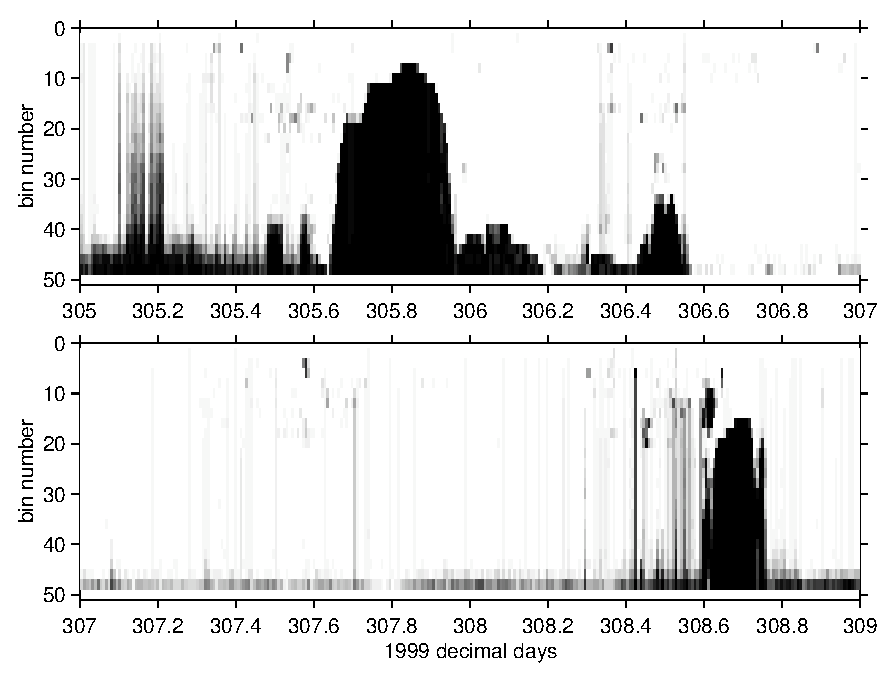
\includegraphics[width=9cm]{pgoodnb}
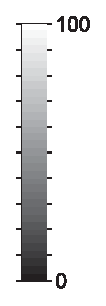
\includegraphics[trim=0 -50 0 0,clip, scale=0.3]{palette}}
\hspace*{2.8cm}\subfigure[]{
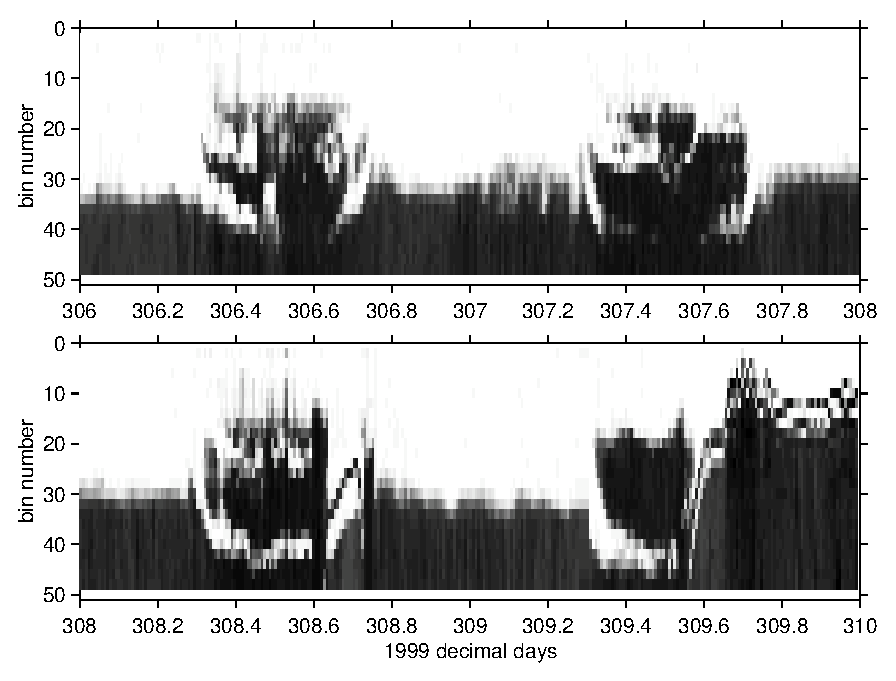
\includegraphics[width=9cm]{pgoodbb}}
\caption{Example of Percentage-good pings vs. time and bin number
for a) 75Khz NB and b) 150Khz BB ADCPs  } \label{fig:winterpgood}
\end{figure}

The comparison between on station and underway of the mean and
standard deviation profiles for the Amplitude and Percentage good
(PG) show a small degradation of the signal while underway
(Fig.~\ref{fig:winterquality}). Similar trends are seen in all
other variables checked. The variability generally increased below
500m for the NB ADCP (e.g. PG) and no deeper data while underway
are used in the chapter. The variability seen in the BB ADCP
increased more rapidly at a shallower depth, 100m, reaching a
maximum saturation at 250m, below which depth the PG falls below
80\% and no data will be used. Data between 100m and 250m are
presented only after careful examination.

A comparison of the two systems was done by a linear regression on
data acquired during a three and a half day drifting experiment
(2-5 November) within the poleward flow core. Data in the depth
range of 54-70m for the NB were compared to data between 51-75m
from the BB for the entire duration of the experiment
(Fig.~\ref{fig:wintercal}). In general, the NB measured greater
velocities than the BB, by 6\% and 13\% on the U and V components
as shown below,
\begin{eqnarray}
  U_{BB} = 0.94\,(\pm 0.03)\times U_{NB} + 0.006\,(\pm 0.004),\\
  \label{eq:adcpcorrU}
  V_{BB} = 0.87\,(\pm 0.03)\times V_{BB} + 0.01 \,(\pm 0.004),
  \label{eq:adcpcorrV}
\end{eqnarray}
with correlations $r^2=0.95,0.92$ respectively. Confidence limits
for the coefficients at 95\% level of confidence are shown in
brackets. Considering the difference in depth resolution and the
2min offset between the two ADCPs, both systems agree well and
data from the BB ADCP will be use to enhance details of the top
200m of the water column. No attempt was done to correct the NB
ADCP data with the calibration as little more information would be
gained considering the high smoothing involved with the CTD data.
\begin{figure}
\centering \subfigure[]{
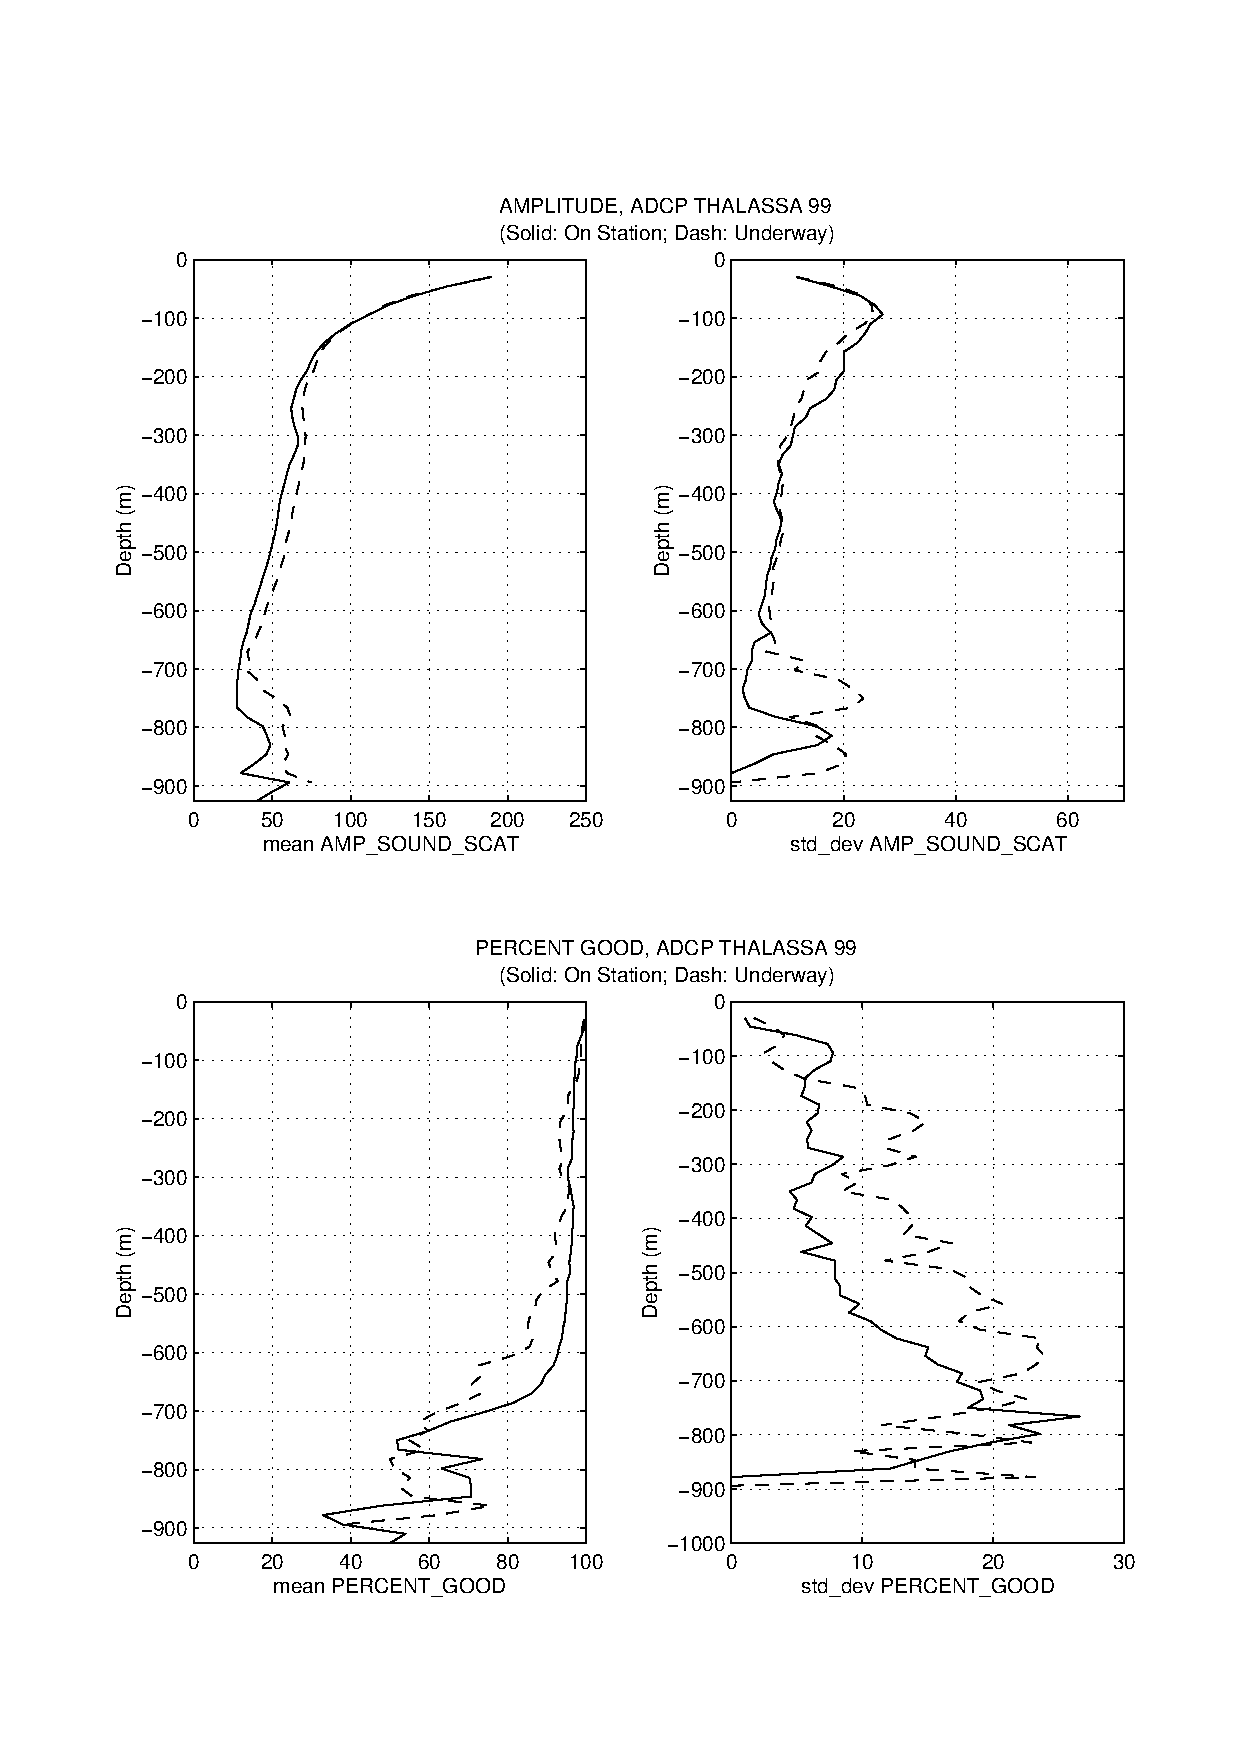
\includegraphics[width=6cm]{qualitynb}}
\subfigure[]{
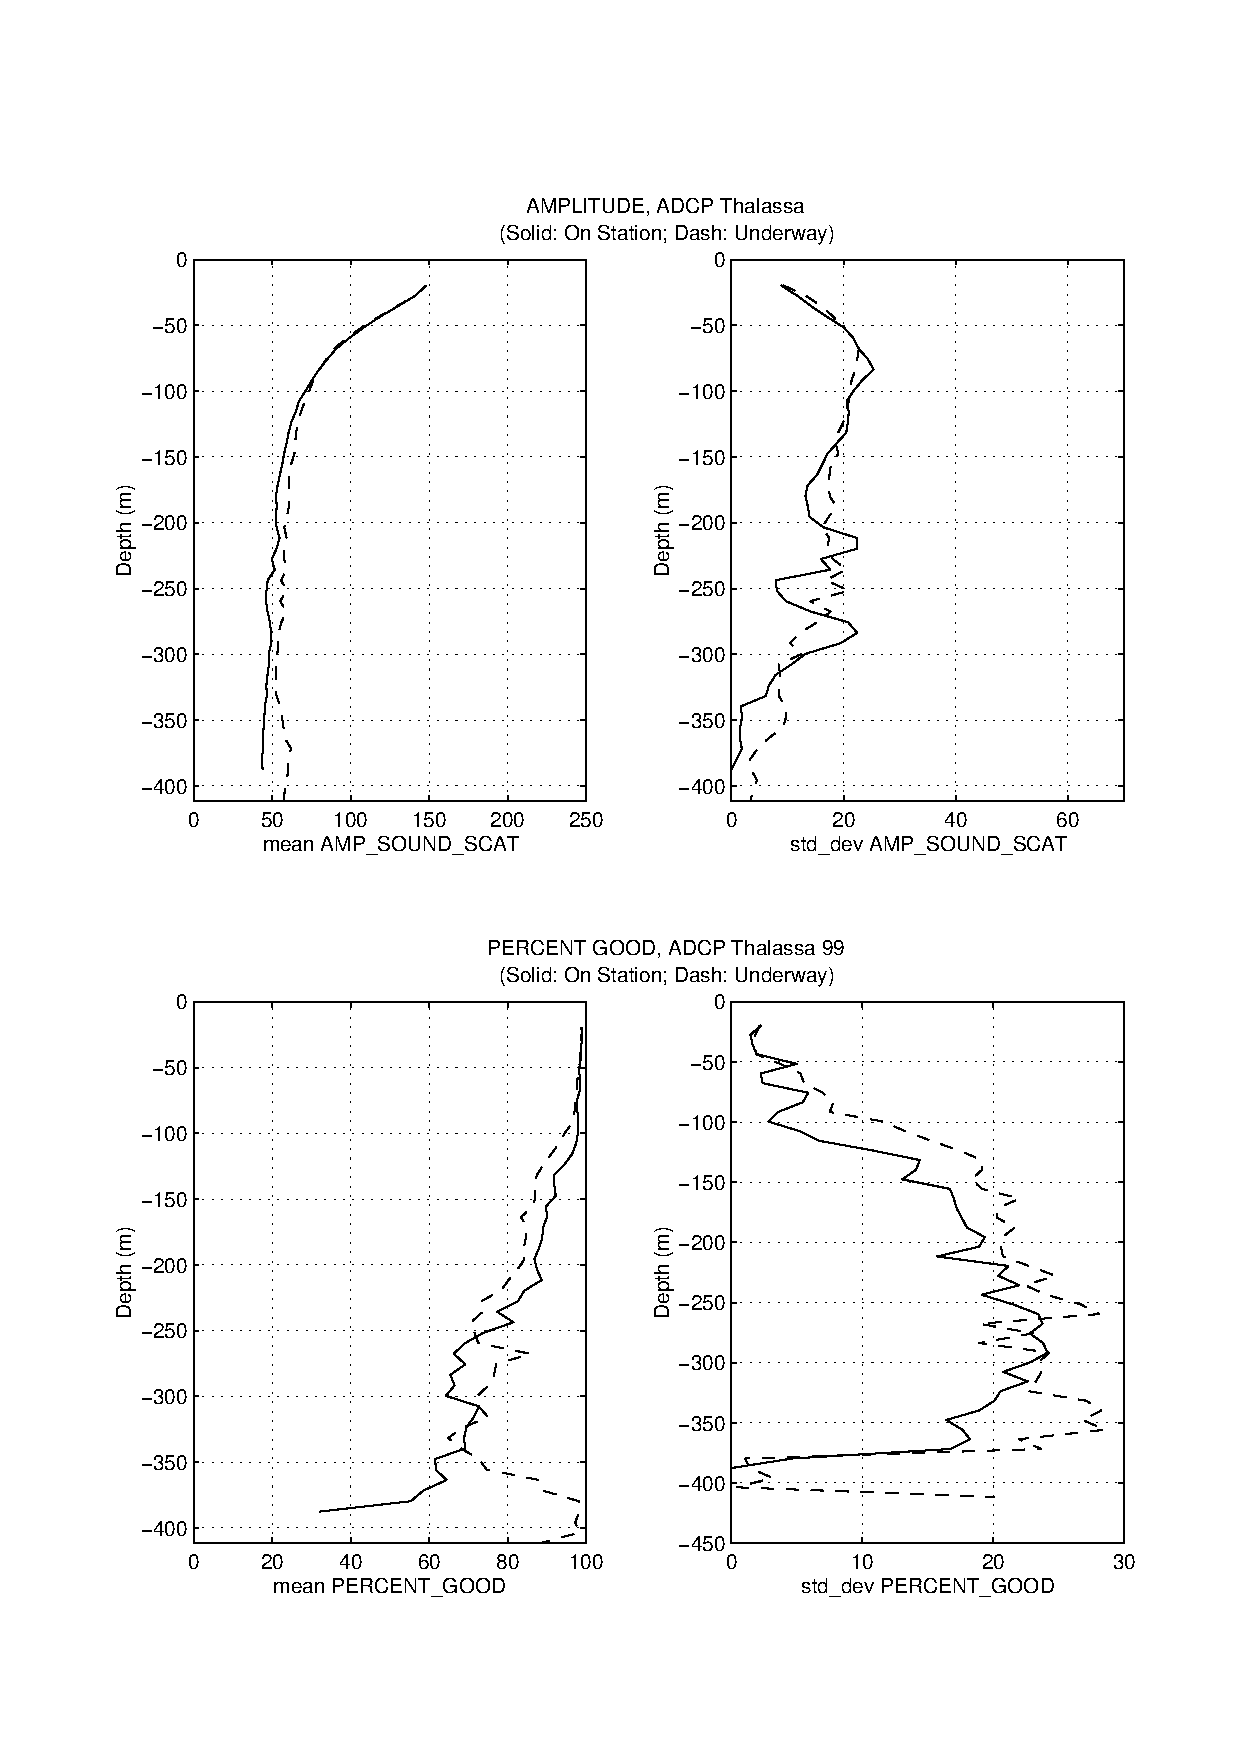
\includegraphics[width=6cm]{qualitybb}}
\caption{Comparison between underway and on station averaged and
standard deviation profiles of Amplitude and Percentage good for
a) 75Khz NB and b) 150Khz BB ADCPs } \label{fig:winterquality}
\end{figure}

\begin{figure}
\centering \subfigure[]{
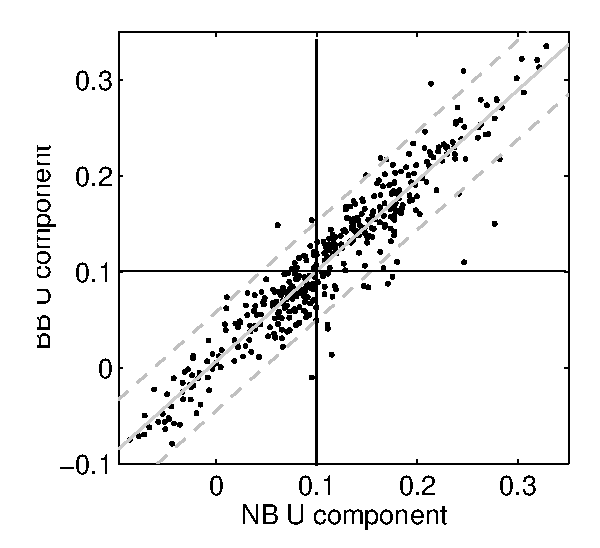
\includegraphics[width=6cm]{ucalibration}}
\subfigure[]{
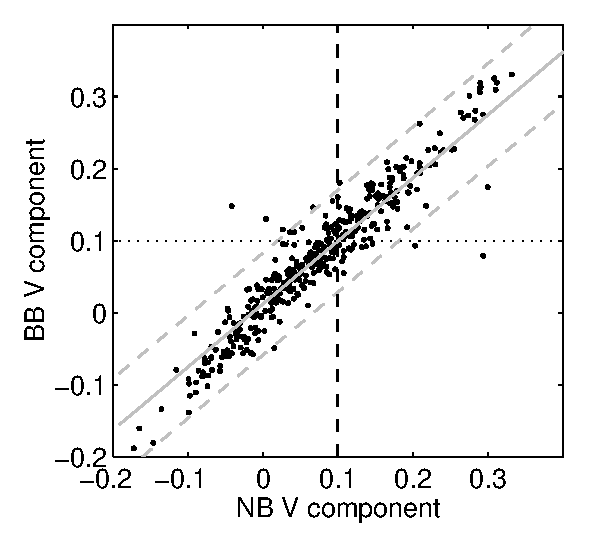
\includegraphics[width=6cm]{vcalibration}}
\caption{Linear Least-square fit and confidence intervals at 95\%
between NB and BB ADCP data during the poleward flow drift
experiment averaged over a depth range of 54-70m and 51-75m
respectively for a) U component and b) V component. Values in
\vel} \label{fig:wintercal}
\end{figure}


\section{Results}
\subsection{Background and evolution}
\begin{figure}
\abajocap \centering \subfigure[Oct 10-16]
{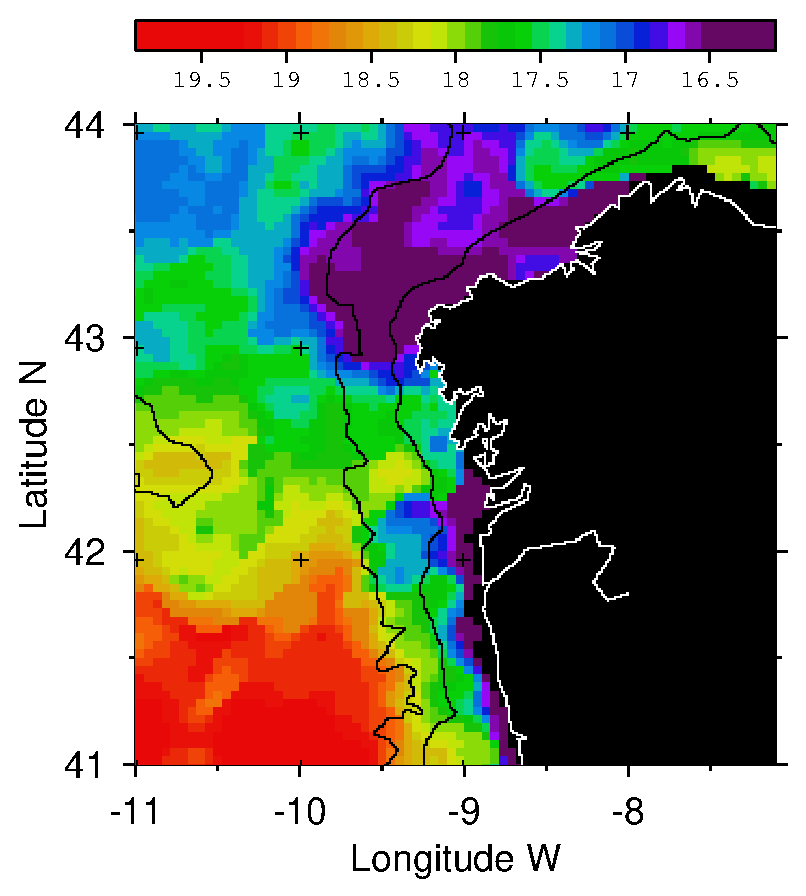
\includegraphics[width=6cm]{oct10-16c}} \subfigure[Oct 17-23]
{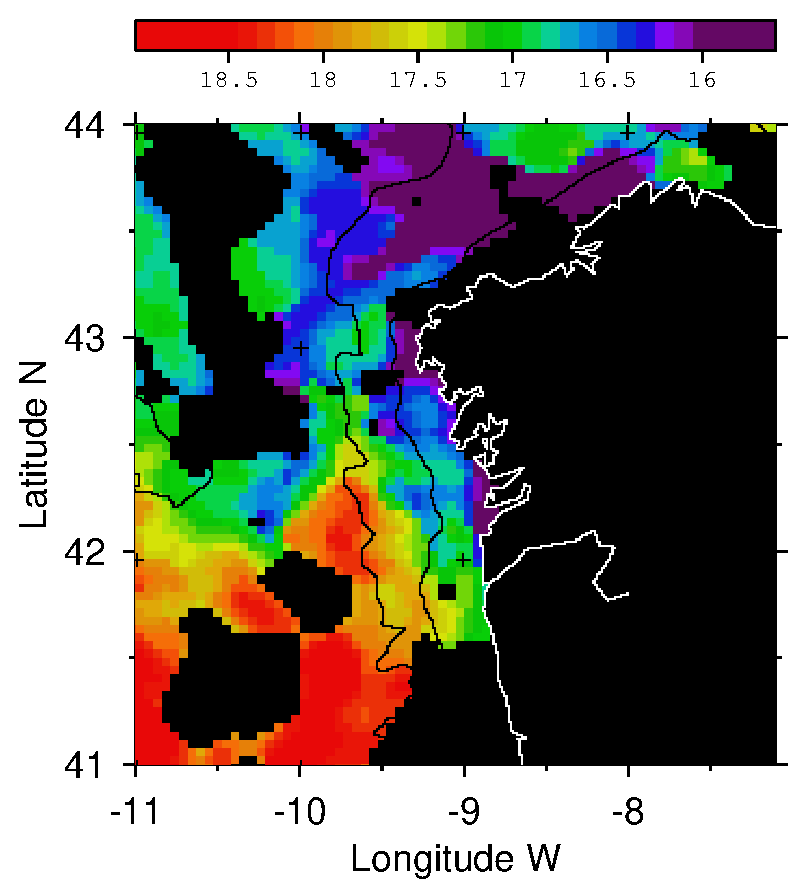
\includegraphics[width=6cm]{oct17-23c}} \subfigure[Oct 24-30]
{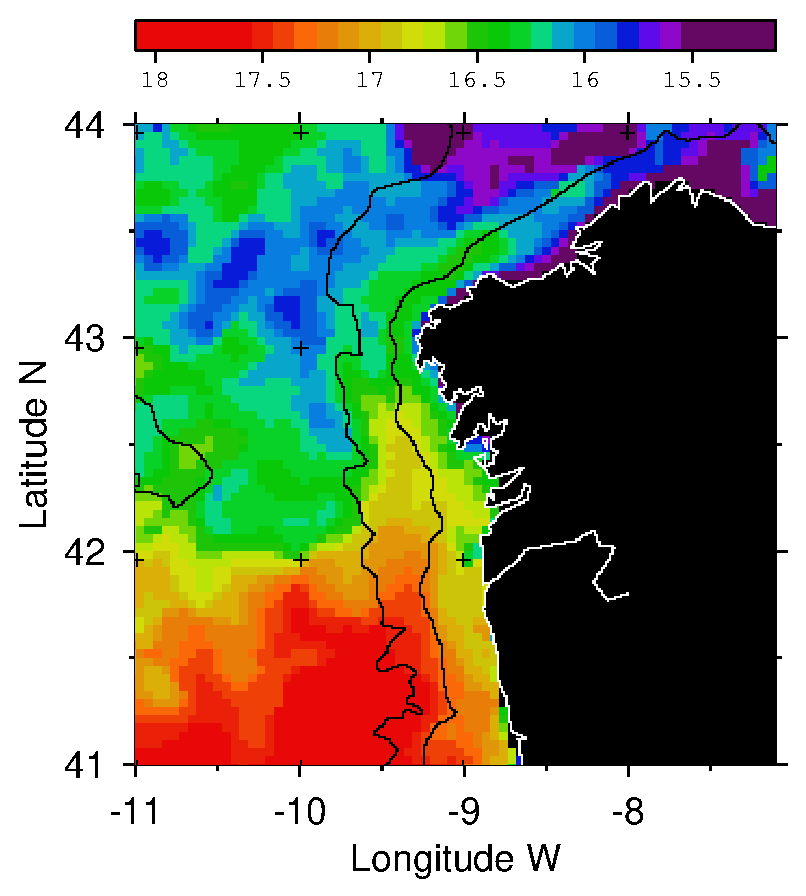
\includegraphics[width=6cm]{oct24-30c}} \subfigure[Oct 31- Nov 6]
{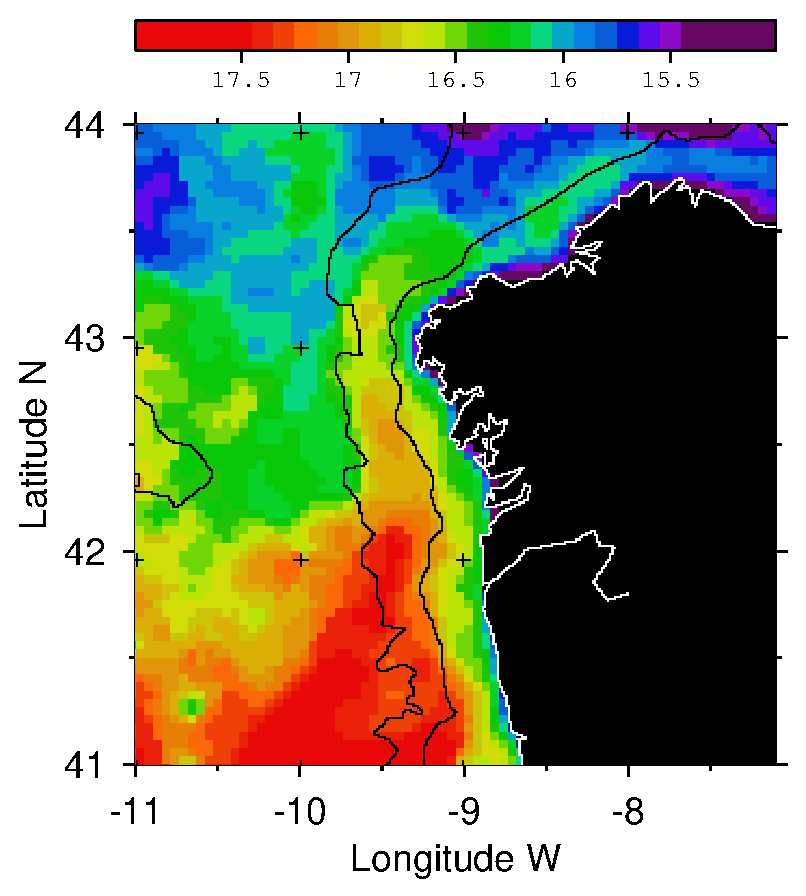
\includegraphics[width=6cm]{oct31-06c}} \caption{Weekly SST
composites during the THAL99 cruise (13 October-7 November 1999).
Clouds and land are masked as black.} \arribacap
\label{fig:thal_sst}
\end{figure}
%PONER UN EJEMPLO DE SST EN TODA LA COSTA IBERICA PARA VER SI HAY
%UN MAXIMO EN EL GRADIENTE DE SST ALREDEDOR DE 40-41, TAMBIEN
%COMPARAR IMAGENES DE SEAWIFFS PARA VER SI EL MAYOR GROSOR DESPUES
%DE FINISTERRE SE DEBE A AGUAS DULCES
%
Weekly composites of SST for the cruise area
(Fig.~\ref{fig:thal_sst}) spanning the entire cruise show the warm
anomaly related to the poleward flow starting to develop at mid
cruise and strengthening towards its end. A general decrease of
1.5\deg C in SST is apparent in the sequence. A meridional SST
gradient of 1\deg C per 10-40km is present in all images, centred
at 42\deg. During the week starting prior to the cruise, evidence
of remnant coastal upwelling can be seen on the west coast and
north of Cape Finisterre (Fig.~\ref{fig:thal_sst}a). Moderate
poleward winds on 14-18 October (see
Fig.~\ref{fig:thal_buoydata}a-b) reduced the coastal band of
upwelled water and a warm intrusion of SST moved northwards along
the 1000m isobath north of 42\deg(Fig.~\ref{fig:thal_sst}b). Winds
increased on 19-23 October and the coastal upwelled water
disappeared from both coasts (Fig.~\ref{fig:thal_sst}c). The warm
intrusion (1\deg warmer than surrounding water on the west coast)
became better defined, its core located between the 200m and 1000m
isobath on the west coast. The intrusion can be tracked around
Cape Finisterre after which it weakened (temperature anomaly of
0.5\deg C) and became closer to the coast. A short upwelling
favourable winds pulse on 26-27 October and 2-3 November could
have been responsible for the narrow band of cold water close to
the west coast, however the warm poleward intrusion became better
defined, with the 1\deg C anomaly reaching Cape Finisterre. North
of the cape, the intrusion had become wider and still proceeded to
move along the coast the following week (not shown) in the face of
upwelling favourable winds (Figs.~\ref{fig:thal_buoydata}).
%\begin{figure}
%\arribacap \centering \subfigure[]
%{\includegraphics[height=4.5cm]{eofthal1}} \subfigure[]
%{\includegraphics[height=4.5cm]{eofthal2}} \caption{Wind CEOF
%amplitudes for a) EOF\#1 and b) EOF\#2 (13 October- 30 November)
%extracted from the analysis in chapter~\ref{ch:winds}. Arrows with
%lighter color indicate the cruise period. Arrow on the right of a)
%indicates the direction of northward winds.}
%\label{fig:thal_winds}
%\end{figure}
\begin{figure}
\arribacap \centering \subfigure[]
{\includegraphics[height=4.8cm]{sillthalwind}} \subfigure[]
{\includegraphics[height=4.8cm]{villthalwind}} \\
\subfigure[] {\includegraphics[height=4.5cm]{sillthalcurr}}
\subfigure[] {\includegraphics[height=4.5cm]{villthalcurr}}
\caption{Wind (a-b) and Current (c-d) vectors measured at buoys
a,c) S and b,d) F (1 October- 30 November). Light gray corresponds
to the cruise period.} \label{fig:thal_buoydata}
\end{figure}

%A subset of the complex amplitude time series from
%Chapter~\ref{ch:winds} for the winter 1999 CEOF analysis including
%the cruise period (Fig.~\ref{fig:thal_winds}) shows two periods of
%sustained downwelling favourable winds, 13-24 October and 29-31
%separated by a four day upwelling favourable period.

Daily median of hourly winds from buoys S and F from 1 October-30
November are shown in Fig.~\ref{fig:thal_buoydata}a-b (see
Fig.~\ref{fig:thal_adcp_st}a for their position) and are
representative of the larger scale winds as measured by the
Seawinds instrument on the QuikScat satellite (see
Chapter~\ref{ch:winds}). No data from buoy N were available for
that period due to failure of the buoy. Maximum upwelling and
downwelling favourable winds of 13\vel were measured at F. The
cruise was characterised by weak SE winds until 15 October,
becoming stronger ($\sim$ 13\vel) and more SW and W towards the 23
October. Winds were highly variable for the remaining of the
cruise with brief pulses alternating upwelling and downwelling
favourable winds. After the cruise, 8-23 November, winds become
upwelling favourable.

Subtidal surface currents (Fig.~\ref{fig:thal_buoydata}c-d) were
southwards at the beginning of the record at S, rotated clockwise
and became poleward from 10 October, prior to the change in winds,
to 7 November. The period included a brief current reversal around
18-19 October, after a weakening of downwelling favourable winds.
Although winds changed afterwards to upwelling favourable,
currents remained poleward with a small offshore component. At F,
currents were larger ($\sim$ 22\velc\, on the 29 October compared
to $\sim$ 15\velc\, at S) but followed the same evolution as at S.
The only difference being the earlier onset of poleward currents
and the near reversal of currents on 8-18 November.

Summarizing, the THAL99 cruise took place during the onset of the
winter poleward flow regime at the end of a weak summer upwelling
regime (see Chapter~\ref{ch:winds}), when persistent poleward flow
started to develop. In the remainder of the chapter, data will be
presented in two sections, the west coast sampling from 13-21
October which can be related to the first stages of the poleward
flow development seen at the buoys; and the north coast sampling,
during which the poleward flow was steadier and stronger and had
reached north of Cape Finisterre.
\begin{table}[th]
  \centering
\begin{tabular}{llllll}
\hline\hline
\multicolumn{1}{c}{Transect} & \multicolumn{1}{c}{Instrument} & \multicolumn{1}{c}{St. Time} & \multicolumn{1}{c}{End Time} & \multicolumn{1}{c}{St. Position} & \multicolumn{1}{c}{End Position} \\
\hline
 S & \multicolumn{1}{c}{CTD} & 14/10 15:22 & 15/10 20:07 & 9\deg\,59-42\deg\,09 & 8\deg\,57-42\deg\,08 \\
 & \multicolumn{1}{c}{} & 14/10 15:38 & 15/10 13:57 & 9\deg\,59-42\deg\,09 & 8\deg\,58-42\deg\,08 \\
S & \multicolumn{1}{c}{ADCP} & 15/10 22:12 & 16/10 02:19 & 9\deg\,12-42\deg\,09 & 10\deg\,00-42\deg\,09 \\
 & \multicolumn{1}{c}{} & 16/10 02:27 & 16/10 07:07 & 9\deg\,58-42\deg\,09 & 9\deg\,8-42\deg\,08 \\
\hline
 & \multicolumn{1}{c}{CTD} & 16/10 14:56 & 17/10 14:37 & 10\deg\,00-42\deg\,40 & 9\deg\,12-42\deg\,40 \\
P & \multicolumn{1}{c}{ADCP} & 16/10 15:57 & 17/10 14:17 & 10\deg\,00-42\deg\,39 & 9\deg\,14-42\deg\,40 \\
 & \multicolumn{1}{c}{} & 18/10 02:43 & 18/10 06:53 & 9\deg\,57-42\deg\,40 & 9\deg\,13-42\deg\,40 \\
\hline
 & \multicolumn{1}{c}{CTD} & 18/10 14:06 & 19/10 11:41 & 10\deg\,01-43\deg\,00 & 9\deg\,18-43\deg\,00 \\
 & \multicolumn{1}{c}{} & 18/10 15:27 & 18/10 21:06 & 9\deg\,59-43\deg\,00 & 9\deg\,24-43\deg\,00 \\
N & \multicolumn{1}{c}{ADCP} & 18/10 22:08 & 19/10 01:35 & 9\deg\,25-43\deg\,00 & 10\deg\,01-43\deg\,00 \\
 & \multicolumn{1}{c}{} & 19/10 01:43 & 19/10 07:23 & 10\deg\,01-43\deg\,00 & 9\deg\,24-43\deg\,00 \\
 & \multicolumn{1}{c}{UOR} & 18/10 22:45 & 19/10 01:35  & 9\deg\,25-43\deg\,00 & 10\deg\,01-43\deg\,00 \\
\hline
 & \multicolumn{1}{c}{CTD} & 25/10 9:54 & 26/10 5:30 & 8\deg\,22-43\deg\,35 & 9\deg\,10-44\deg\,32 \\
PW1 & \multicolumn{1}{c}{} & 21/10 10:25 & 21/10 23:52 & 8\deg\,27-43\deg\,34 & 9\deg\,30-44\deg\,55 \\
 & \multicolumn{1}{c}{ADCP} & 22/10 03:12 & 22/10 14:13 & 9\deg\,29-44\deg\,54 & 7\deg\,56-43\deg\,50 \\
 & \multicolumn{1}{c}{} & 25/10 09:40 & 26/10 05:58 & 8\deg\,25-43\deg\,40 & 9\deg\,10-44\deg\,32 \\
\hline
PW2 & \multicolumn{1}{c}{CTD} & 31/10 8:12 & 31/10 22:06 & 8\deg\,50-44\deg\,00 & 8\deg\,50-43\deg\,24 \\
 & \multicolumn{1}{c}{ADCP} & 31/10 09:39 & 31/10 22:59 & 8\deg\,50-44\deg\,01 & 8\deg\,50-43\deg\,24 \\
 & \multicolumn{1}{c}{} & 31/10 23:09 & 01/11 04:46 & 8\deg\,49-43\deg\,24 & 8\deg\,50-44\deg\,07 \\
\hline
PW3 & \multicolumn{1}{c}{CTD/ADCP} & 01/11 11:48 & 01/11 22:47 & 8\deg\,49-43\deg\,24 & 9\deg\,30-43\deg\,42 \\
\hline
PW4 & \multicolumn{1}{c}{CTD/ADCP} & 02/11 8:17 & 02/11 19:58 & 9\deg\,31-43\deg\,42 & 9\deg\,18-43\deg\,08 \\
\hline\hline
\end{tabular}\caption{Time, location and instrument of the transects
sampled during cruise Thal99.}\label{tb:wintertran}
\end{table}
\FloatBarrier
\subsection{The west coast}

During Leg A, three transects were sampled, S, P and N. They were
occupied with CTD stations once, and repeated at least one more
time with ADCP and on occasions with the UOR. Details of all
transect times, starting and ending points are summarised in
Table~\ref{tb:wintertran}. CTD transect plots were built through
Barnes interpolation with scales 10m and 15km in the vertical and
horizontal respectively, with no extrapolation, i.e. the start and
end points of each plot correspond to a CTD cast. We have used
distance from the shelf edge, as identified from the ADCP signal,
with positive values offshore from the shelf as the horizontal
gridding variable. Due to the larger station separation offshore,
the interpolation scheme smooths horizontal gradients. Unsmoothed
surface salinity and temperature from the Thermosalinometer have
been included to help assess the level of smoothing.

CTD section plots of transect S show low surface salinity and
temperature values of 35.3psu and 17.2\deg-17.5\deg C
(Fig.~\ref{fig:thalCTD_S}a-b) extending from nearshore to 13km
from the shelf edge. Offshore surface temperature and salinity
values increased to 18.7\deg C and 35.75psu in a sharp surface
layer front of $\sim$5km (Figs.~\ref{fig:thalCTD_S}a-b). The low
surface salinity layer nearshore was 50m deep
(Figs.~\ref{fig:thalCTD_S}c) with associated high fluorescence
levels (Fig.~\ref{fig:thalCTD_S}e) indicative of a freshwater
origin. Nonetheless, the slight coastal uplifting of all isolines
(salinity, temperature and density) provides evidence of weak
coastal upwelling though no isolines break the surface nearshore.
The surface front also marked the transition between a surface
fluorescence maximum inshore and the subsurface fluorescence
maximum centred at 50m offshore (Figs.~\ref{fig:thalCTD_S}e). This
deepening of the maximum could be related with the seaward
intrusion of offshore warm surface waters, as indicated by buoy S
at the time (Fig~\ref{fig:thal_buoydata}c), which have not been in
contact with coastal waters. This idea is supported by the
association of the offshore subsurface maxima with relatively low
salinity values at 40-50m (Fig~\ref{fig:thalCTD_S}c).
\begin{figure}[t]
\arribacap \centering %
\subfigure[]{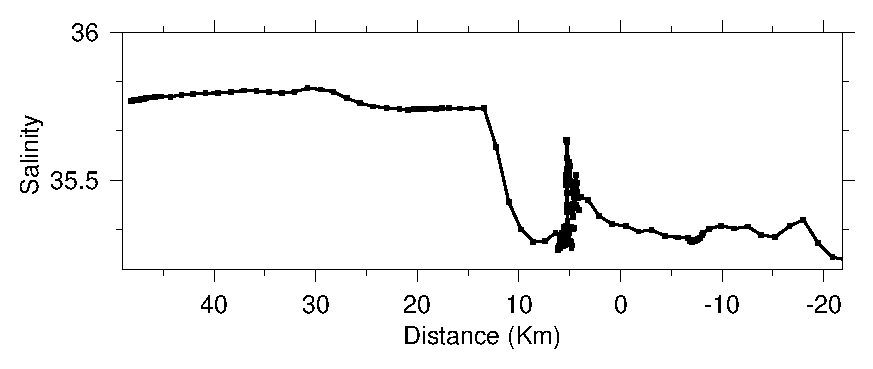
\includegraphics[height=2.2cm]{THS1_S}}\hspace{0.2cm}
\subfigure[]{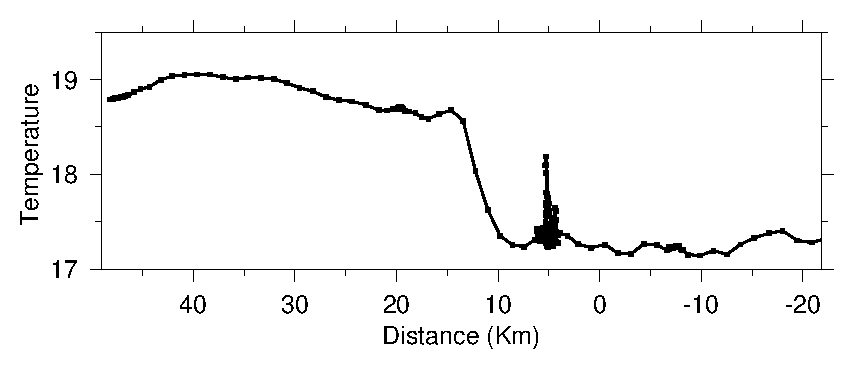
\includegraphics[height=2.2cm]{THS1_T}}\quad%
\subfigure[]{\includegraphics[height=5cm]{S_S}}%
\subfigure[]{\includegraphics[height=5cm]{S_T}}\quad%
\subfigure[]{\includegraphics[height=5cm]{S_F}}%
\subfigure[]{\includegraphics[height=5cm]{S_D}}%
\caption{Transect S CTD sections (14-15 October) for a) surface
salinity, b)surface temperature, and vertical sections of c)
salinity, d) temperature, e) fluorescence and e) density.}
\label{fig:thalCTD_S}
\end{figure}

A subsurface salinity maximum ($>$35.9psu) was measured at 65-110m
depth, 0-35km off the shelf. It was related to a localised
increase in vertical separation of the isotherms
(Fig~\ref{fig:thalCTD_S}d). At that level, isopycnals (e.g 27.1
isopycnal) deepened towards the coast, which would be indicative
of geostrophic poleward flow (Fig~\ref{fig:thalCTD_S}f). In
contrast, below 400m higher salinity was measured within 30km of
the shelf in relation to the northward advection of Mediterranean
water. Due to the wide spacing of the stations it is difficult to
estimate the offshore limit of the subsurface intrusion although
some indication can be gained from the more densely spaced ADCP
dataset.
\begin{figure}[t]
\arribacap \centering %
\subfigure[]{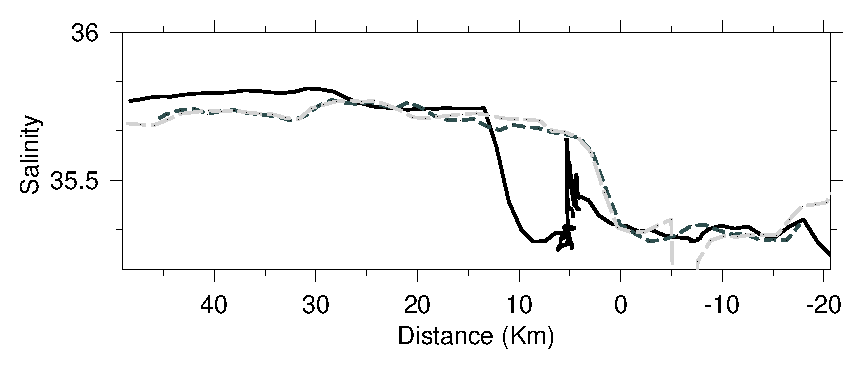
\includegraphics[height=2.8cm]{THS_S}}\hspace*{0.4cm}
\subfigure[]{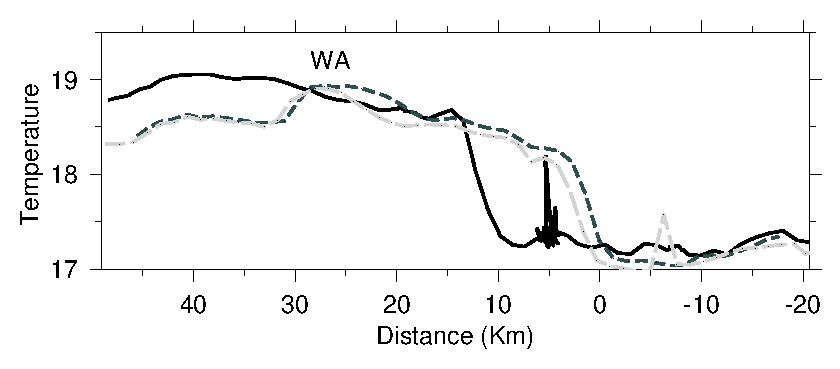
\includegraphics[height=2.8cm]{THS_T}}\quad%
\subfigure[]{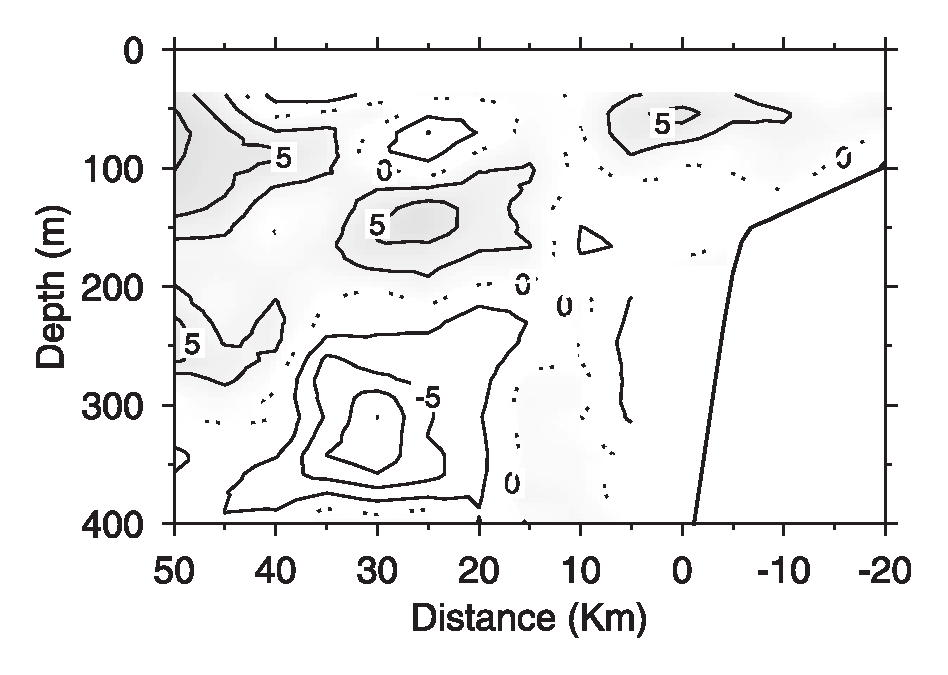
\includegraphics[height=5cm]{allS2_4_rotufinal}}%
\subfigure[]{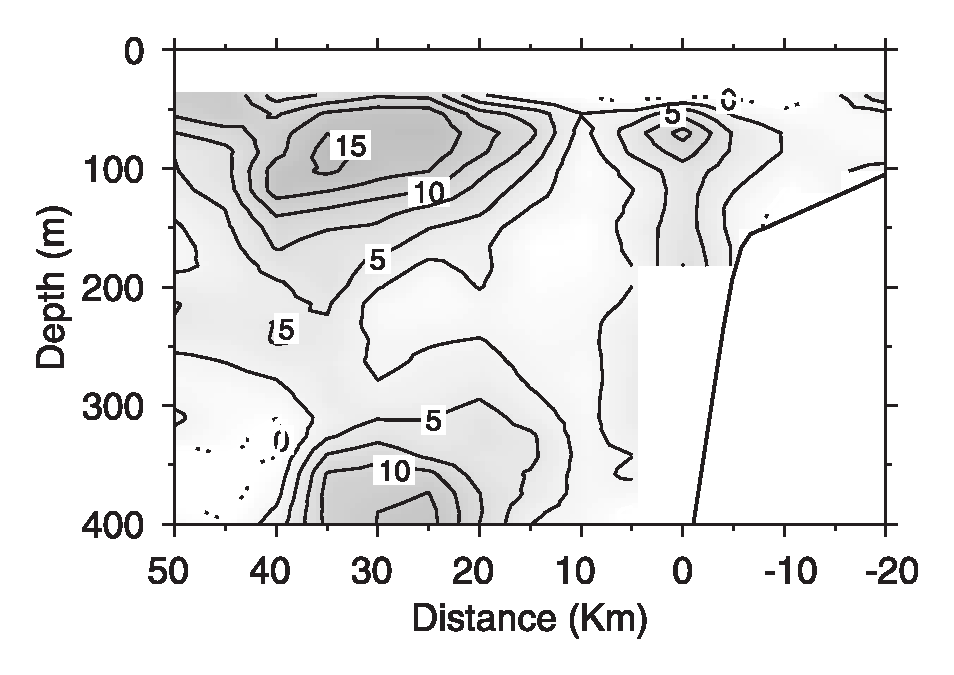
\includegraphics[height=5.5cm]{allS2_4_rotvfinal}}%
\caption{All surface a) salinity and b) temperature coincident
with the ADCP sections (lighter dashed line indicates later
crossing) for transect S. The developing warm anomaly (WA) is
labelled. NB ADCP averaged sections, c) across-shelf component
(+ve onshore) and d) along-shelf component (+ve northward)}
\label{fig:thalADCP_S}
\end{figure}

The U and V velocity components have been rotated throughout into
along and across-shelf components. The choice of the along-shelf
direction is difficult, particularly in an area of such a complex
bathymetry. Uncertainties in the along-shelf direction will have
an important effect on the across-shore component which should be
taken with caution. Mean sections of the along and across-shelf
velocity components (Fig.~\ref{fig:thalADCP_S}) for the three
repetitions of transect S (see table~\ref{tb:wintertran}) have
been built in an attempt to reduce the tidal signal. More
effective and complex methods exist for reducing the tidal signal
in shipboard ADCP records
\citep[e.g.][]{Candela92,Howarth92,Munchow00a} but the
availability of repeated sections and the strength of the offshore
residual currents in comparison to the tidal flow
\citep[$\sim$8\velc,][]{Fanjul97} allowed us to use the simplest
method.

During the ADCP repeat surveys, the surface salinity and
temperature (Fig.~\ref{fig:thalADCP_S}a-b) showed a shoreward
advection of 10km of the frontal region. Also, a surface
temperature maximum (temperature anomaly of $\sim$0.5\deg C))
developed at 20-30km from the shelf edge (WA in
Fig.~\ref{fig:thalADCP_S}b). The across-shelf component
(Fig.~\ref{fig:thalADCP_S}c) was small and overall onshore, except
for a deep offshore flowing core at 200-400m centred  at 30km off
the slope. The along-shelf component (Fig.~\ref{fig:thalADCP_S}d)
revealed two northward cores offshore of the shelf reaching speeds
of 15-10\velc, coincident with minima in the standard deviation
($\sigma <$ 5\velc not shown). The shallower, at 50-120m depth,
was 10km offshore of the surface temperature maximum at 25km off
the shelf (Fig.~\ref{fig:thalADCP_S}b) measured in the last two
repetitions of the transect. It also corresponded in position with
the interpolated offshore limit of the subsurface salinity maximum
in Fig.~\ref{fig:thalCTD_S}c. The deeper core appears shifted
shorewards with respect to the shallower one and could be related
to the northward advection of Mediterranean water. A weaker
northward flowing core can also be seen on the shelf edge
occupying most of the water column.

\begin{figure}[t]
\arribacap \centering %
\subfigure[]{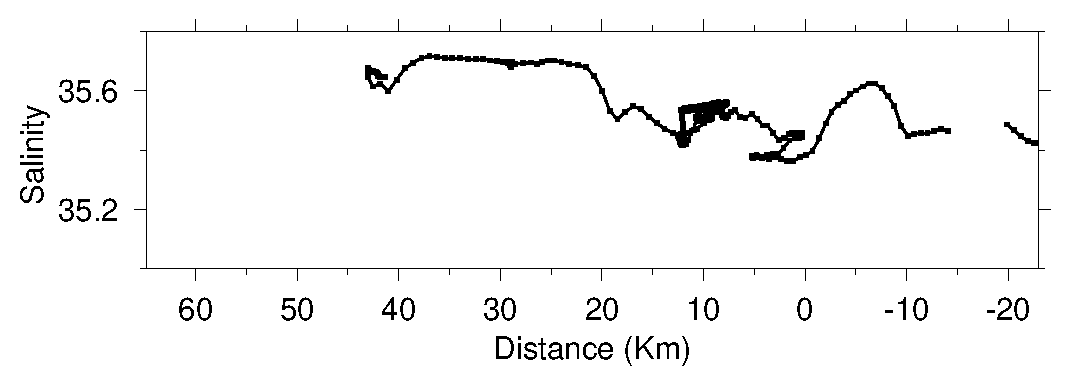
\includegraphics[height=2.2cm]{THP1_S}}\hspace{0.2cm}
\subfigure[]{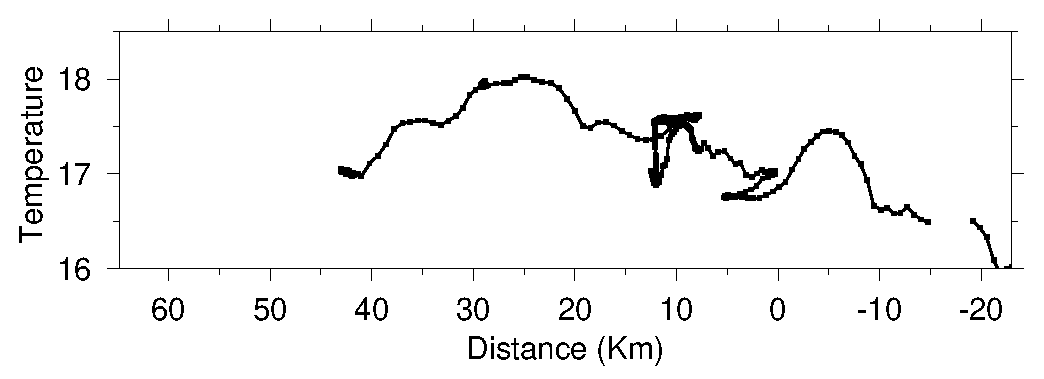
\includegraphics[height=2.2cm]{THP1_T}}\quad%
\subfigure[]{\includegraphics[height=5cm]{P_S}}%
\subfigure[]{\includegraphics[height=5cm]{P_T}}\quad%
\subfigure[]{\includegraphics[height=5cm]{P_F}}%
\subfigure[]{\includegraphics[height=5cm]{P_D}}%
\caption{Transect P CTD sections (16-17 October)  for a) surface
salinity, b)surface temperature, and vertical sections of c)
salinity, d) temperature, e) fluorescence and e) density.}
\label{fig:thalCTD_P}
\end{figure}

Transect P (Fig~\ref{fig:thalCTD_P}) showed similar
characteristics to transect S. A surface temperature maximum of
18\deg C was measured at 25km off the shelf
(Fig~\ref{fig:thalCTD_P}b), 1\deg C less than transect S. The
salinity also reached a maximum of 35.7psu between 20-40km off the
shelf edge (Fig~\ref{fig:thalCTD_P}a) but was $\sim$0.1psu less
saline than in transect S. The surface thermosalinograph record
showed weaker T and S fronts on this section than in transect S,
but over the outer shelf small maxima in both T and S were
evident. The low salinity layer nearshore was shallower, reached
25m depth, and had higher values than in transect S, reflecting
the larger concentration of freshwater sources further south (The
Rias Bajas and the Mi\~{n}o river).

The subsurface salinity maximum at 50-150m depth spanned the
entire section with a weak local maximum  at 30km offshore
(Fig~\ref{fig:thalCTD_P}c), where the temperature increased
locally (Fig~\ref{fig:thalCTD_P}d). Similar to transect S, the
surface fluorescence maximum was deeper underneath the warm tongue
intrusion (Fig~\ref{fig:thalCTD_P}e). On the shelf between
10-15km, all isolines showed a local increase in vertical
separation below 50m depth at the same time that fluorescence
levels increased near the bottom inshore and on the shelf edge
(Fig~\ref{fig:thalCTD_P}e). The latter could be an indications of
a bottom Ekman layer associated with poleward flow in the shelf.

Surface temperature and salinity in the two repetitions of
transect P (Fig~\ref{fig:thalADCP_P}~a-b) showed a shoreward
displacement of the offshore warm intrusion and front similar to
Fig~\ref{fig:thalADCP_S}~a-b. In response to the sustained if weak
downwelling winds the warm anomaly was better defined with a local
maximum temperature around 25km offshore of over 18\deg C in the
first section and slightly cooler in the second section. The
narrower warm and salty intrusion on the shelf also moved further
inshore possibly in response to the downwelling winds. The
averaged velocity section showed weak onshore velocities
(Fig~\ref{fig:thalADCP_P}~c) which agreed with the general
shoreward displacement of the surface structures. The alongshore
component (Fig~\ref{fig:thalADCP_P}~d) was predominantly poleward
both off and on the shelf ($>$10\velc) and like transect S, a
subsurface maximum of $\sim$20\velc\, at 50m depth 30km off the
shelf was again associated with the offshore end of the warm
intrusion.
\begin{figure}[t]
\arribacap \centering \hspace*{-0.2cm}%
\subfigure[]{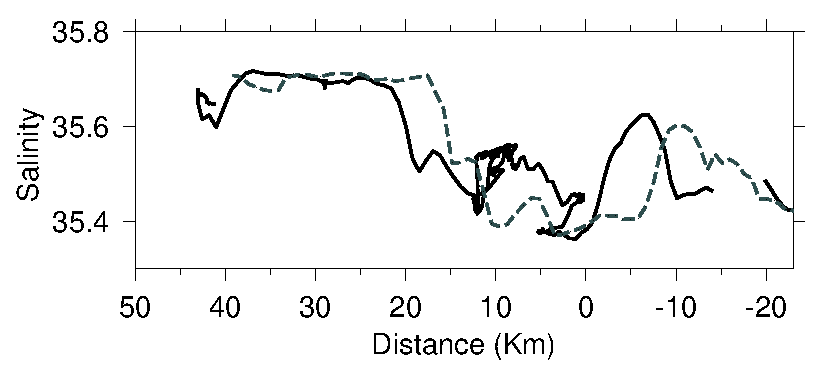
\includegraphics[height=2.9cm]{THP_S}}\hspace*{0.1cm}
\subfigure[]{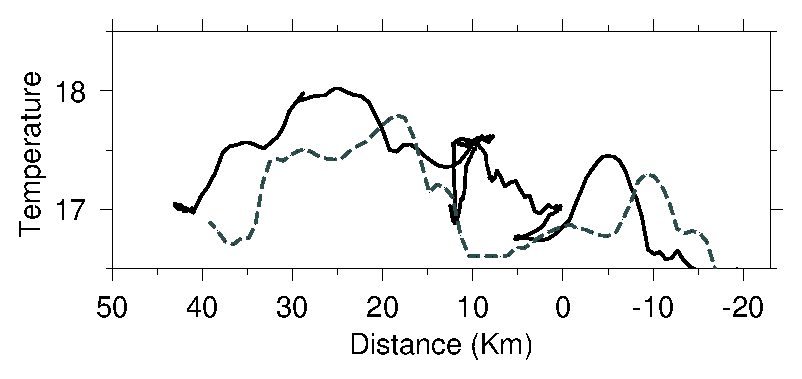
\includegraphics[height=2.9cm]{THP_T}}\hspace*{0.8cm}\\
\subfigure[]{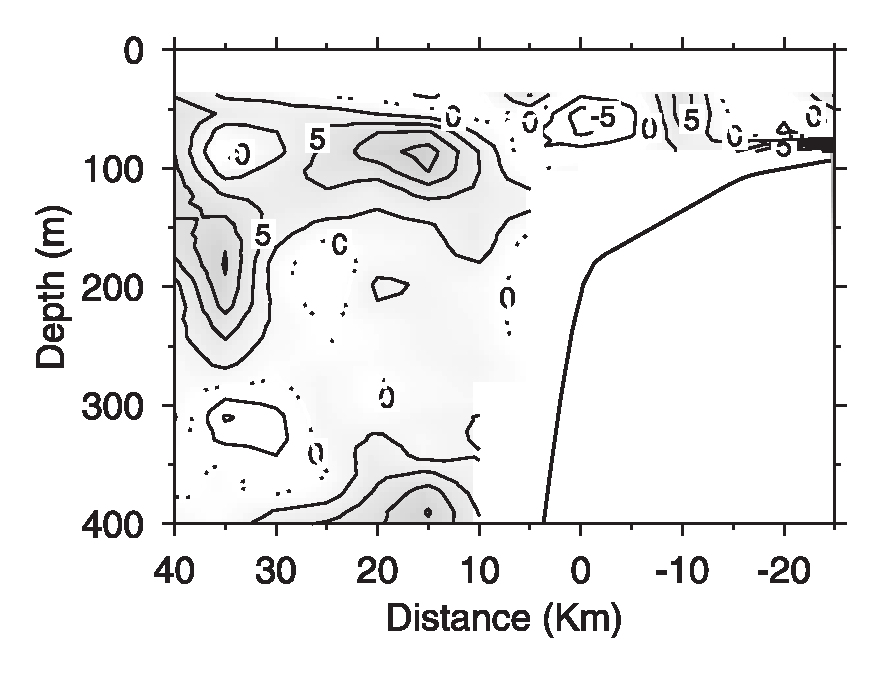
\includegraphics[height=5cm]{P6_8_rotufinal}}\hspace*{0.5cm}%
\subfigure[]{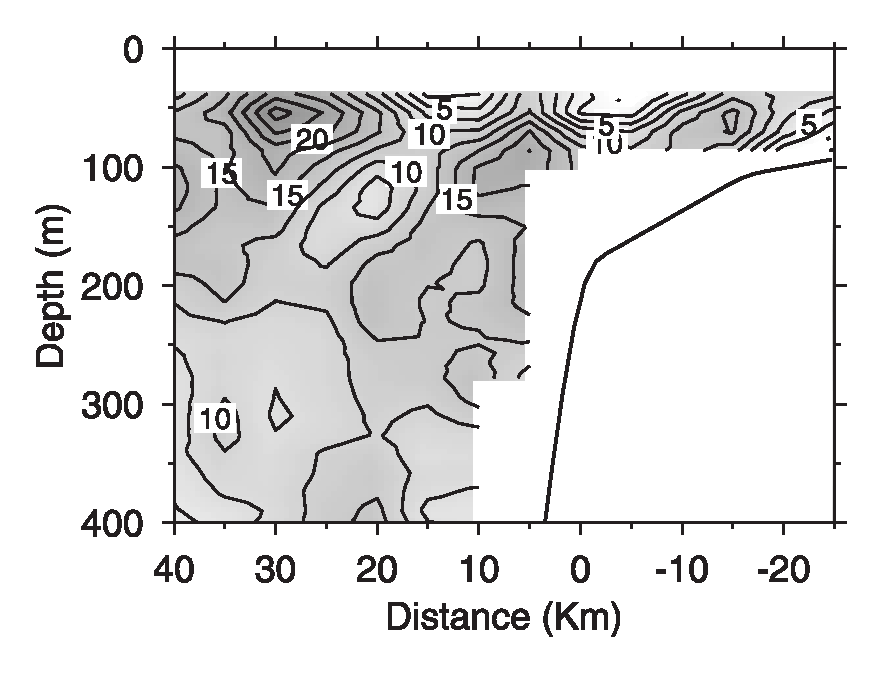
\includegraphics[height=5cm]{P6_8_rotvfinal}}%
\caption{All surface a) salinity and b) temperature coincident
with the NB ADCP section averages (lighter dashed line indicates
later crossing) for transect P: c) across-shelf component (+ve
onshore) and d) along-shelf component (+ve northward)}
\label{fig:thalADCP_P}
\end{figure}

Transect N (Fig~\ref{fig:thalCTD_N}) showed similar
characteristics to the previous ones: a warm surface intrusion
associated with low fluorescence values,  a subsurface salinity
maximum at 100m off shelf and low salinity waters associated with
freshwater runoff on the shelf. The surface signature of the
offshore warm and salty intrusion (Fig~\ref{fig:thalCTD_N}a-b) is
less well defined than in transect P. The colder and fresher shelf
waters form a front at the shelf break similar to transect S
albeit not as sharp. Freshwater runoff is present on the shelf
forming a thicker (50m) and narrower layer than in more southern
transects although it still extended to the shelf edge. As in
transect P, the isotherms and isopycnals on the shelf separated
vertically between 30-200m (Fig~\ref{fig:thalCTD_N}d,f), and again
bottom fluorescence values increased on the shelf edge compared to
transect S (Fig~\ref{fig:thalCTD_N}e), suggesting sinking along
the shelf bottom. Two cores of subsurface salinity maxima
(Fig~\ref{fig:thalCTD_N}b) are clearly discernible, one on the
shelf and one offshore.
\begin{figure}[t]
\arribacap \centering %
\subfigure[]{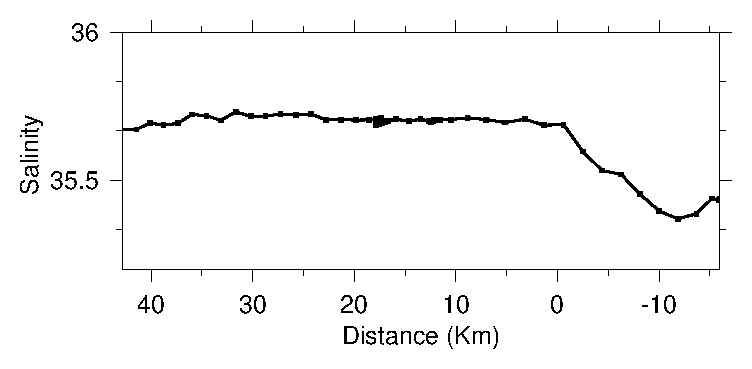
\includegraphics[height=2.2cm]{THN1_S}}\hspace{0.2cm}
\subfigure[]{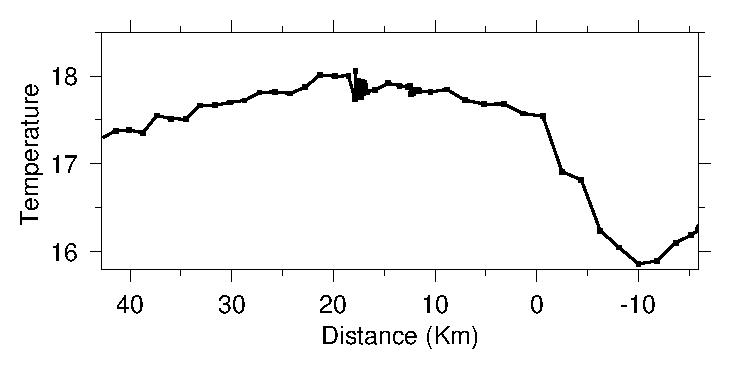
\includegraphics[height=2.2cm]{THN1_T}}\quad%
\subfigure[]{\includegraphics[height=5cm]{N_S}}%
\subfigure[]{\includegraphics[height=5cm]{N_T}}\quad%
\subfigure[]{\includegraphics[height=5cm]{N_F}}%
\subfigure[]{\includegraphics[height=5cm]{N_D}}%
\caption{Transect N CTD sections (18-19 October)  for a) surface
salinity, b)surface temperature, and vertical sections of c)
salinity, d) temperature, e) fluorescence and e) density.}
\label{fig:thalCTD_N}
\end{figure}
The evolution of the surface salinity and temperature
(Fig.~\ref{fig:thalADCP_N}a-b) during subsequent repetitions of
transect N showed an enhancement of the warm intrusion temperature
signature but little shoreward displacement in contrast with the
previous transects. The velocity structure of the averaged section
showed offshore flow west of 20km (Fig.~\ref{fig:thalADCP_N}c)
with negligible associated along shelf component while poleward
flow (Fig.~\ref{fig:thalADCP_N}d) was associated with zero or very
weak onshore flow. Barotropic poleward flow was measured on the
shelf ($>$15\velc\, in both ADCPs), and off the shelf in two cores
similar to transect S although they were weaker. The shallower
core had peak velocities of $\sim$6-7\velc\, extending from the
shallower bin to 200m depth at 30km off the shelf. The deeper core
had velocities in excess of 7\velc\, at 300m depth, 20km off the
shelf. Overall maximum velocities were weaker and closer to the
shelf break than in transect S.

\begin{figure}[t]
\arribacap \centering \hspace*{-0.3cm}%
\subfigure[]{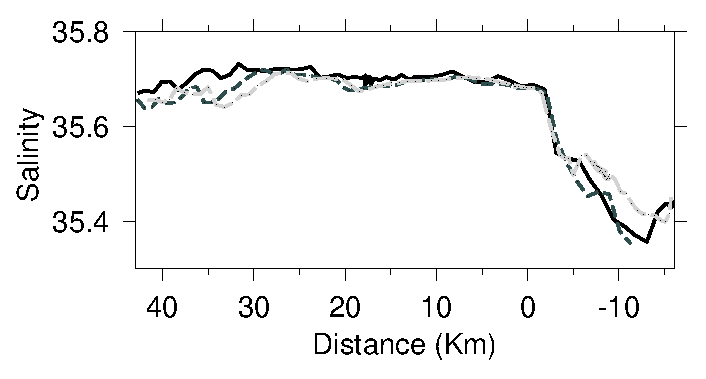
\includegraphics[height=3.1cm]{THN_S}}\hspace*{0.2cm}
\subfigure[]{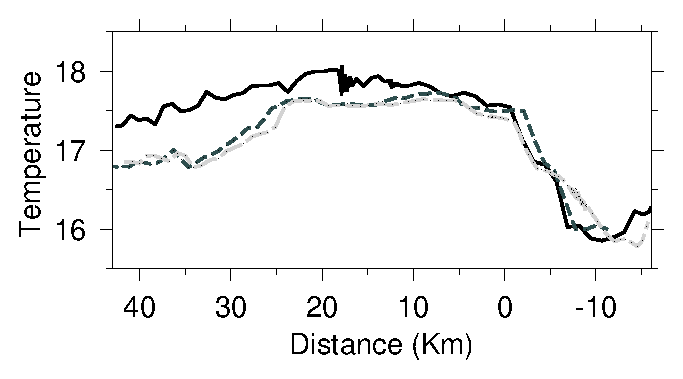
\includegraphics[height=3.1cm]{THN_T}}\hspace*{-0.7cm}\\
\subfigure[]{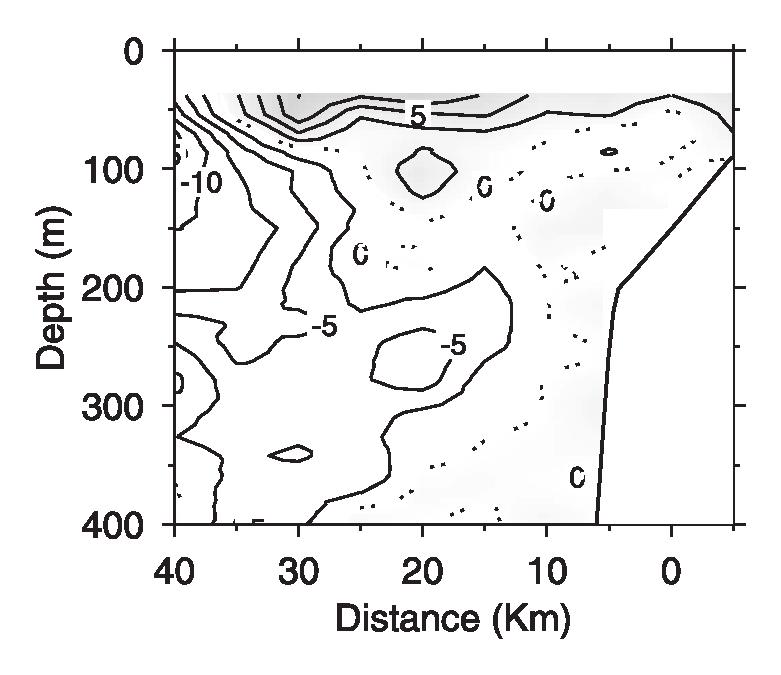
\includegraphics[height=5cm]{allN10_12_rotufinal}}\hspace*{0.2cm}%
\subfigure[]{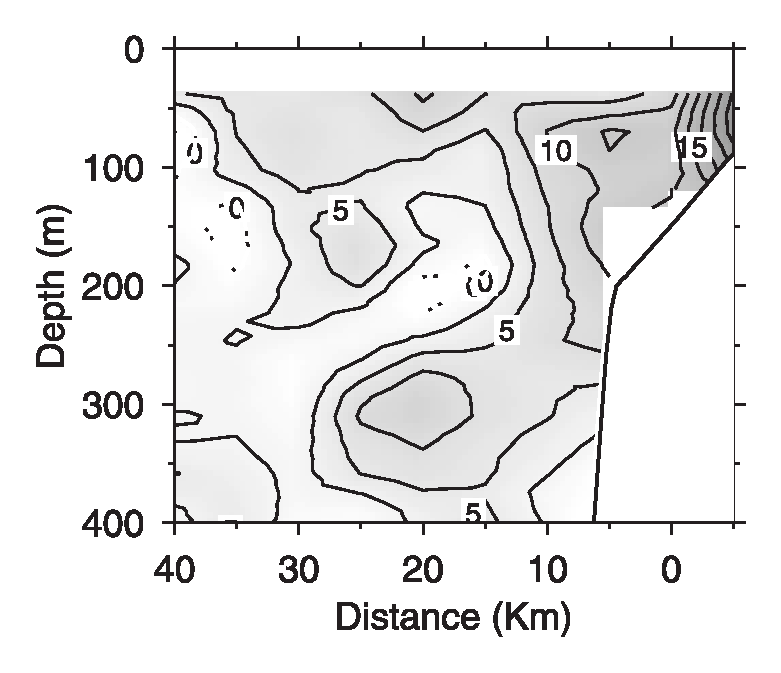
\includegraphics[height=5cm]{allN10_12_rotvfinal}}%
\caption{All surface a) salinity and b) temperature coincident
with the NB ADCP section averages (lighter line colour indicates
later crossing) for transect N: c) across-shelf component (+ve
onshore) and d) along-shelf component (+ve northward)}
\label{fig:thalADCP_N}
\end{figure}
The second repetition of transect N (Fig.~\ref{fig:thalADCP_N})
with UOR and BB ADCP shows the detailed vertical structure of the
warm intrusion (Fig.~\ref{fig:thalUOR_N}). It is worth pointing
out the numerous vertical fluctuations at the thermocline (larger
than 15m) indicative of the high internal wave activity of the
region \citep{Barton01}. The intrusion is very shallow affecting
mainly the top 50m, and is characterised by a widened thermocline
(Fig.~\ref{fig:thalUOR_N}a). The narrow core ($\sim$20km) had
temperatures in excess of 17.5\deg C in agreement with the surface
records in Fig.~\ref{fig:thalADCP_N}b. The velocity structure in
Fig.~\ref{fig:thalADCP_N}b largely reflected northward flow in the
thermal anomaly. Maximum speeds in the strongly baroclinic flow
were associated with the offshore limit of the intrusion, and was
near zero at its nearshore end.

\subsubsection{Summary}
\begin{figure}[t]
\arribacap \centering
\subfigure[]{\includegraphics[height=5cm]{uorN_T}}\\
\subfigure[]{\includegraphics[height=5cm]{uorN_V}}%
\caption{Coincident N section of a) temperature from the UOR and
b) along-shelf component (+ve northward) from the BB ADCP.}
\label{fig:thalUOR_N}
\end{figure}

A surface N-S gradient in temperature was evident from the data
between transects S and P. Surface values decreased by 1\deg C.
Similar structures were seen in all three transects. Less saline
water was encountered over the shelf and was bounded by a strong
surface front at the shelf edge. Evidence for upwelling was seen
only in the earliest sampled transect S. At deeper levels,
isolines separated vertically and an increase in fluorescence
along the bottom of the shelf suggested that a bottom Ekman layer
associated with poleward flow on the shelf was producing offshore
flow down the sloping bottom. A surface warm anomaly with reduced
fluorescence levels developed during the cruise, generally inshore
of the subsurface salinity maxima. Its western end was associated
with a local velocity maximum $>$10\velc. The subsurface salinity
maximum was invariably present between 20 and 30km offshore of the
shelf break at 70-120m depth, although its maximum deepened
northwards. Poleward flow was present in all sections both off and
on the shelf.

\subsection{The North Coast}
The data presented here were collected between 25 October and 6
November, during a period of variable winds
(Fig.~\ref{fig:thal_buoydata}a-b) but strong and steady poleward
flow off both the west coast and Cape Finisterre
(Fig.~\ref{fig:thal_buoydata}c-d), with surface values
$>$15\velc\, at the buoy locations. Underway data in transect PW1
were collected in the north coast on 21 and 22 October but strong
swell prevented CTD sampling.

The first CTD sampling of transect PW1 (the easternmost transect
in the north coast) on the 25-26 October was undertaken before the
core of the poleward flow reached the site
(Fig~\ref{fig:thal_sst}c). The surface values of salinity and
temperature (Fig.~\ref{fig:thalCTD_PW1}a and b) showed no warm
anomaly indicative of the poleward intrusion seen in the west
coast. A band of low salinity water was measured at -20km inshore
of the shelf-break although there was no associated temperature
change. However, a surface temperature minimum was located at the
shelf break. The subsurface maximum of salinity
(Fig.~\ref{fig:thalCTD_PW1}c) associated with the poleward flow in
the west coast was again present in the data although its maximum
was weaker (35.8psu instead of 35.9psu in the western coast) and
closer to the shelf edge (within 10km) at 100m. The isohalines
deepened at the shelf edge, as in previous transects P and N. The
salinity maximum ($>$35.7psu) extended offshore 70km and down to
300m depth. Transects in the west coast did not reach as far
offshore and it remains unknown whether a similar distribution,
with a clear offshore limit, was present. At the deepest levels
($>$400m) salinity was relatively high nearshore, but decreased to
$<$35.6psu at 65km offshore. The lowest salinity ($<$35.3psu) was
measured in the near-surface layer above 25-30m, between the
shelf-break and 55km offshore. This was probably in response to
the brief upwelling favourable winds on 25-26 October and
represents offshore advected Ria's water.
\begin{figure}[t]
\begin{widefig}{-.5cm}{-.7cm}
\arribacap \centering \hspace{0.4cm}
\subfigure[]{\includegraphics[height=2.0cm]{THGC1_S}}\hspace{0.4cm}
\subfigure[]{\includegraphics[height=2.0cm]{THGC1_T}}\quad%
\subfigure[]{\includegraphics[height=4.5cm]{GC1_S}}%
\subfigure[]{\includegraphics[height=4.5cm]{GC1_T}}\quad%
\subfigure[]{\includegraphics[height=4.5cm]{GC1_F}}%
\subfigure[]{\includegraphics[height=4.5cm]{GC1_D}}%
\caption{Transect PW1 CTD sections (25-26 October)  for a) surface
salinity, b)surface temperature, and vertical sections of c)
salinity, d) temperature, e) fluorescence and e) density.}
\label{fig:thalCTD_PW1}
\end{widefig}\end{figure}

The vertical temperature structure (Fig.~\ref{fig:thalCTD_PW1}d)
follows the salinity distribution. Lower temperatures were
associated with low salinity at the surface. The subsurface
salinity maximum corresponds to locally warmer waters (seen as
deepening of the 12\deg C isotherm) and reduced mixed layer depth
in agreement with its southern origin where wind mixing is weaker
and near surface stratification stronger. Two cores were apparent
in this subsurface warm anomaly at 60 and 10km offshore. The
thermocline deepened sharply at the shelf edge reaching the bottom
at -15km inshore and a similar vertical gradient was maintained
shorewards. At the deepest levels, the offshore low salinity
waters were colder than the saltier waters closer to the slope
which mark the shallowest levels of Mediterranean water influence.

High surface fluorescence levels (Fig.~\ref{fig:thalCTD_PW1}e)
were measured across the entire section except for the coastal
stations inshore of -10km. There, the water was vertically mixed
(Fig.~\ref{fig:thalCTD_PW1}f). No sign of reduced surface
fluorescence levels were found in relation with the poleward
intrusion in contrast with all west coast sections.

The vertical density distribution (Fig.~\ref{fig:thalCTD_PW1}f)
strongly resembled the temperature structure with deeper mixed
layers at either side of the subsurface maximum salinity and steep
deepening of the isopycnals at the shelf edge indicative of
geostrophic poleward flow.


\begin{figure}[ht]
\begin{widefig}{-.5cm}{-.7cm}
\arribacap
\hspace*{-3.8cm}\includegraphics[width=4cm]{PW1_stations}\\
\centering
\subfigure[]{\includegraphics[width=7.cm]{THGC1all_S}}\hspace*{0.4cm}
\subfigure[]{\includegraphics[width=7.cm]{THGC1all_T}}\quad%
\subfigure[]{\includegraphics[width=7.cm]{GC1_1_Urot}}\hspace*{0.4cm}
\subfigure[]{\includegraphics[width=7.cm]{GC1_1_Vrot}}\quad%
\subfigure[]{\includegraphics[width=7.cm]{GC1_3_Urot}}\hspace*{0.4cm}
\subfigure[]{\includegraphics[width=7.cm]{GC1_3_Vrot}}%
\caption{Location of all surface realisations of PW1 transect
(21-26 October, lighter line colour indicates later crossing) with
, a) salinity and b) temperature, and first and last vertical
sections of rotated velocity components c) along and d)across
shelf (21 October),  e) along and f) across shelf (25-26
October).} \label{fig:thalADCP_PW1}
\end{widefig}\end{figure}

The evolution of surface salinity and temperature with the
measured ADCP sections of PW1 is shown in
Fig.~\ref{fig:thalADCP_PW1}. The weekly composite of SST around
the time of the first two crossings (Fig.~\ref{fig:thal_sst}b)
shows a band of cold water at the location of transect PW1,
remnant of previous upwelling events, and indeed a band of cold
and salty water was seen in the \emph{in situ} data over the shelf
(Fig.~\ref{fig:thalADCP_PW1}a-b). The coastal band increased in
temperature inshore which supports the idea of inactive upwelling.
By the third crossing, fresher and warmer water (salinity
$<$35.4psu, temperature $>$16\deg C) was established nearshore
(20km inshore of the shelf edge). Surface temperature and salinity
decreased overall. Changes in the velocity sections
(Fig.~\ref{fig:thalADCP_PW1}c-f) suggest an increase in poleward
flow nearshore with flows reaching 30\velc\, on the last crossing
(Fig.~\ref{fig:thalADCP_PW1}f). Much of the variability present in
the sections (particularly in the across-shore component, but also
in the alongshore one) is tidal, but the strength of the flow and
its similarities to the hydrography (Fig.~\ref{fig:thalCTD_PW1})
give support to the presence of a largely barotropic coastal
poleward flow.

\begin{figure}[t]
\arribacap \centering %
\subfigure[]{\includegraphics[height=2.3cm]{THPW1_S}}\hspace{0.2cm}
\subfigure[]{\includegraphics[height=2.3cm]{THPW1_T}}\quad%
\subfigure[]{\includegraphics[height=5cm]{PW1_S}}%
\subfigure[]{\includegraphics[height=5cm]{PW1_T}}\quad%
\subfigure[]{\includegraphics[height=5cm]{PW1_F}}%
\subfigure[]{\includegraphics[height=5cm]{PW1_D}}%
\caption{Transect PW2 CTD sections (31 October)  for a) surface
salinity, b)surface temperature, and vertical sections of c)
salinity, d) temperature, e) fluorescence and e) density.}
\label{fig:thalCTD_PW2}
\end{figure}

The next three transects PW2-4, were done consecutively towards
Cape Finisterre (Fig.~\ref{fig:thal_adcp_st}b) in the presence of
downwelling favourable winds (Fig.~\ref{fig:thal_buoydata}). The
surface profile consistently displayed uniform salinity offshore
($\sim$ 35.6psu e.g. Fig.\ref{fig:thalCTD_PW2}a), a weak surface
maximum between 10 and 30km off the shelf
(Fig.~\ref{fig:thalCTD_PW4}a), and a minimum of 34.4psu on the
shelf (Fig.\ref{fig:thalCTD_PW4}a). The temperature field was
characterised by an across-shore gradient with maximum
temperatures nearshore
(Figs.~\ref{fig:thalCTD_PW2}a-\ref{fig:thalCTD_PW4}a) and no sign
of a surface warm anomaly, in contrast with the situation found in
the west coast.

The low salinity coastal band (5km inshore of the shelf edge) was
vertically homogeneous and extended to the bottom (down to 100m)
at the common coastal station in the first two transects
(Figs.~\ref{fig:thalCTD_PW2}-\ref{fig:thalCTD_PW3}a). It probably
came from the three rivers that flow into the Ria of Betanzos (see
Fig.~\ref{fig:thal_adcp_st}). In transect PW4 it showed lower
surface salinity and formed a shallow layer (top 25m). A gradual
change in the subsurface salinity maximum was seen in all
transects (Figs.~\ref{fig:thalCTD_PW2}-\ref{fig:thalCTD_PW4}). As
the sections were sampled closer to Cape Finisterre the salinity
maximum (delimited by the 35.7psu isohaline) broadened, deepened
to 350m depth near the slope, and broached the surface between 5
and 30km off the shelf (Fig.~\ref{fig:thalCTD_PW4}c). It
intersected the bottom 10km either side of the shelf edge. The
salinity maximum also increased in value to $>$35.9psu towards
Cape Finisterre becoming shallower from 100m to 65m at 30-20km
offshore.

\begin{figure}[ht]
\arribacap \centering %
\subfigure[]{\includegraphics[height=2.3cm]{THPW2_S}}\hspace{0.1cm}
\subfigure[]{\includegraphics[height=2.3cm]{THPW2_T}}\quad%
\subfigure[]{\includegraphics[height=5cm]{PW2_S}}%
\subfigure[]{\includegraphics[height=5cm]{PW2_T}}\quad%
\subfigure[]{\includegraphics[height=5cm]{PW2_F}}%
\subfigure[]{\includegraphics[height=5cm]{PW2_D}}%
\caption{Transect PW3 CTD sections (1 November)  for a) surface
salinity, b)surface temperature, and vertical sections of c)
salinity, d) temperature, e) fluorescence and e) density.}
\label{fig:thalCTD_PW3}
\end{figure}
\FloatBarrier

The temperature structure of transects PW2-PW4 showed a weakening
of the vertical gradient, seen as wider separation of isotherms
associated with the salinity maximum at 20-30km off the shelf
(Figs.~\ref{fig:thalCTD_PW2}d-\ref{fig:thalCTD_PW4}d). The
intrusions were less apparent in the fluorescence distribution.
Surface values were relatively high ($>$ 0.7 V) along the entire
extension of the sections
(Figs.~\ref{fig:thalCTD_PW2}e-\ref{fig:thalCTD_PW4}e), but
decreased towards Cape Finisterre. A local maximum existed at
10-20km offshore in all sections, in contrast with the west coast
transects, and nearshore in PW2 and PW3
(Figs.~\ref{fig:thalCTD_PW2}e-\ref{fig:thalCTD_PW3}e). In
transects PW3 and PW4, a local minimum existed on the shelf which
was more pronounced near Cape Finisterre
(Fig.~\ref{fig:thalCTD_PW4}e). The density distribution
(Figs.~\ref{fig:thalCTD_PW2}f-\ref{fig:thalCTD_PW4}f) also showed
vertical separation of isopycnals at the salinity maximum,
particularly in transects PW3 and PW4, and lower density
associated with the coastal freshwater band similar to PW1. They
all suggested geostrophic poleward flow on the shelf and between
100-300m at which depth the isopycnals deepened towards the slope
(Figs.~\ref{fig:thalCTD_PW3}-\ref{fig:thalCTD_PW4}f).

\begin{figure}[t]
\arribacap \centering %
\subfigure[]{\includegraphics[height=2.3cm]{THPW3_S}}\hspace{0.2cm}
\subfigure[]{\includegraphics[height=2.3cm]{THPW3_T}}\quad%
\subfigure[]{\includegraphics[height=5cm]{PW3_S}}%
\subfigure[]{\includegraphics[height=5cm]{PW3_T}}\quad%
\subfigure[]{\includegraphics[height=5cm]{PW3_F}}%
\subfigure[]{\includegraphics[height=5cm]{PW3_D}}%
\caption{Transect PW4 CTD sections (2 November)  for a) surface
salinity, b)surface temperature, and vertical sections of c)
salinity, d) temperature, e) fluorescence and e) density.}
\label{fig:thalCTD_PW4}
\end{figure}

\begin{figure}[t]
\arribacap \centering %
\subfigure[]{\includegraphics[width=7cm]{allPW_rotufinal}}%
\subfigure[]{\includegraphics[width=7cm]{allPW_rotvfinal}}\quad%
\caption{NB ADCP section averages of transects PW2-PW4,  a)
across-shelf component (+ve onshore) and b) along-shelf component
(+ve) northward.} \label{fig:thalADCP_PW24}
\end{figure}

The averaged velocity structure for transects PW2-PW4
(Fig.~\ref{fig:thalADCP_PW24}) shows fundamental differences with
the west coast transects. The across-shelf component
(Fig.~\ref{fig:thalADCP_PW24}a) was offshore weak throughout
($<$7.5\velc) except for a weak onshore narrow area on the shelf
edge. The along-shelf component lacked the double core structure
of the west coast. Instead, coastally trapped along-shelf flow was
in the poleward sense at all levels resembling the area of
salinity larger than 35.8 of Fig.~\ref{fig:thalCTD_PW3}c. Inshore,
a strong baroclinic poleward jet ($>$30\velc) was associated with
the salinity front at the shelf edge.

The last three days of the cruise were dedicated to a short
Lagrangian experiment during 3 14:17-6 11:27 November. A buoy
drogued at 100m with a cruciform sail was placed at the centre of
the poleward flow at 25km offshore coincident with the offshore
salinity maximum of transect PW3 (Fig.~\ref{fig:thalCTD_PW3}c, see
Fig.~\ref{fig:thal_adcp_st}b for the location of the CTD stations
during the drift, D in the graph). The buoy was followed as it
covered, approximately, the distance between transects PW3 and
PW2. Both ADCP's performed well, yielding data down to their
maximum penetration depth, 250m and 650m for the BB and NB
respectively. Mean velocity profiles, rotated to along and
across-shelf components, during the drift and temperature and
salinity profiles for the first and last CTD casts are shown in
figure \ref{fig:thalADCP_PW32}. The velocity profiles
(Fig.~\ref{fig:thalADCP_PW32}a) show continuous poleward flow at
all depths. Maximum discrepancy between the two instruments at
their common depth range was less than 1\velc\, at depths of rapid
change. The across-shelf component (with values $<$4\velc\,
throughout) suggests a three layer structure. The top 200m
corresponds to a strongly sheared poleward flow with an offshore
tendency (that is, with respect to the large scale shelf-edge
orientation on the north coast). Maximum poleward flow (15\velc)
was measured below the thermocline (Fig.~\ref{fig:thalADCP_PW32}b)
at 65m decreasing almost linearly to 8\velc\, at 150m. Along-shelf
poleward flow with near zero across-shelf component can be seen in
the layer between 200m and 400m. The along-shelf component
decreased linearly from 9\velc\, to 7\velc. Below that, between
400m and 550m, weak, slightly offshore poleward flow was again
present.

The three layer velocity structure is less clear in the
temperature and salinity profiles during the drift, showing no
obvious correspondence (Fig.~\ref{fig:thalADCP_PW32}b). The top
layer roughly corresponds to the salinity maximum, which thickened
towards the end of the drift to reach 150m, where a sharp decrease
in salinity (0.08psu) marks it lower limit. The intermediate layer
was characterised by a linearly decreasing salinity and
temperature layer, which showed no differences at the start and
end of the drift. Below 350m, the largest differences between the
first and last CTD of the drift were measured, with both salinity
and temperature decreasing.
\begin{figure}[t]
\arribacap \centering %
\subfigure[]{\includegraphics[width=5cm]{meandriftfinal}}%
\subfigure[]{\includegraphics[width=5cm]{B1-B9}}\quad%
\caption{a)Mean profile of along-shore (grey) and across-shore
(black) components during the drift experiment on 3 14:17-6 11:27
November for both the BB (circles) and NB (solid) ADCP. The three
layers referred to in the text are shown. b) temperature (dashed)
and salinity (solid) for the first (black) and last (grey) CTD of
the drift.} \label{fig:thalADCP_PW32}
\end{figure}

\subsection{Watermass analysis}
\begin{figure}[t]
\arribacap \centering %
\subfigure[]{\includegraphics[width=6cm]{thal99_ts}}%
\subfigure[]{\includegraphics[width=5cm]{ts_pos}}\quad%
\caption{a)T/S diagram between surface and 500m of representative
sub-regions (offshore, coastal and poleward flow) encountered
during the cruise on the west and north coasts. The regions are
color coded as shown in the graph. Circles correspond to the
northernmost CTD cast within each group and asterisks to the
southernmost. b) Position of CTD casts with the same color code as
a).} \label{fig:thal_TS}
\end{figure}

T/S characteristics for the cruise from surface to 500m are
summarized in Fig.~\ref{fig:thal_TS}. Selected casts from offshore
positions outside the poleward flow (red and orange) represent the
background oceanic conditions. They show an increased proportion
of \enawp with respect to the poleward flow casts (green and
yellow) but no consistent differences can be drawn with respect to
their latitude or proximity to the slope (the differences between
the two northernmost offshore cast (red) were the largest). Above
the central waters definition lines, salinity was uniform and no
sign of subsurface salinity maximum was found. It is worth noting
that the central waters T/S relationships were shifted towards
higher salinity or lower temperature compared to the \enaw
reference line \citep{Rios92}. Similar variability in the region
has been linked to decadal changes in the \enawp ventilation
conditions \citep{Perez95,Pollard96} but evidences exist that the
changes are a large scale phenomenon \citep{Huthnance02}. The
poleward flow casts had a larger proportion of \enawt as expected
from its northward advection and a relatively well defined
subsurface salinity maximum on the \enawt definition line. The
subsurface salinity maximum shows similar range at both the west
and north coast as expected from the developing stages of the
poleward flow regime. On the north coast, higher values were
encountered near Cape Finisterre decreasing polewards (eastwards)
reflecting the southern source area at this developing stages.
Surface T/S characteristics away from strong freshwater influences
were very similar among nearshore, offshore and poleward flow
stations which clustered between 35.5-35.7psu and 15.5-16.5\deg C.
The nearshore stations (blue and cyan) showed influences of
freshwater origin ranging from thin freshwater plumes to
vertically mixed shelf-freshwater waters as described in previous
sections. \FloatBarrier
\section{Discussion}
Slope poleward flows are ubiquitous along the entire western
European shelf during at least part of the year. Remotely sensed
SST \citep[e.g.][]{Pingree90}, Lagrangian
\citep[e.g.][]{VanAken02,Pingree93a} and modelling studies
\citep[e.g.][]{Coelho02,New01}, all suggest a continuous flow
originating in the Portuguese coast and ending in the Norwegian
one. In the Iberian Peninsula, the poleward slope current has a
strong seasonality with maximum flow in winter, reversing to
southward flow during the summer
\citep[e.g.][]{Haynes90,Huthnance02}. North of Spain, seasonal
variations in the flow decrease with latitude, with current
reversals in February-April as far north as the Porcupine Bank,
north of the Celtic Shelf \citep{Pingree90}, but only weakening of
the flow in the Hebridean Shelf off Scotland during the summer
\citep{Souza01}. Maximum but more variable poleward flow occurs
during winter in response to stronger winds.

In this chapter, data from the early stages of the slope current
development in autumn have been presented. Favourable winds before
the start of the cruise maintained weak upwelling in a nearshore
band in the west coast and over a broader area off the north
coast, as seen in SST images (Fig.~\ref{fig:thal_sst}a). Winds
were downwelling favourable during the first half of the cruise
and variable during the remainder of the cruise. Downwelling winds
are expected to force poleward currents nearshore (see also
Chapter~\ref{ch:spring}). \citet{Vitorino02} showed that surface
and bottom currents at 41.3\deg N in mid-shelf were highly
correlated to winds, which they lagged by 6h. The expected
poleward wind driven currents on the west coast shelf were
enhanced by the vertical mixing of the low salinity upper layer in
the inner shelf. The increase in vertical mixing is evident in
transects S, P and N during the downwelling winds, where the
surface layer depth increased from 25m to 50m, and reached 100m in
the north coast. There, the thermocline, which occurred between
50m and 80m depth off the shelf, intersected the upper slope
topography as a bottom front, inducing poleward geostrophic flow.
In response to both direct wind forcing, through momentum transfer
and sea level elevation at the coast as a result of onshore Ekman
transport associated with the downwelling winds, and the afore
mentioned wind mixing induced geostrophic flow, poleward velocity
increased over the shelf during the cruise. Velocity less than
2.5\velc\, in the first transect S (Fig.~\ref{fig:thalADCP_S}d),
increased to values larger than 25\velc\, in the final one
(Fig.~\ref{fig:thalADCP_PW24}d). Similar velocities were found by
\citet{Vitorino02}, who measured northward velocities of about
20-30\velc\, in the northern Portuguese shelf during winter, and
\citet{Haynes90} who measured northward velocities at 100m depth
of $\sim$20\velc at 42.8\deg N in September 1986.

The SST images at the time of the cruise showed a meridional SST
gradient around 42\deg N which turned northwards at the slope
forming a warm tongue that progressed northwards as in
\citet{Haynes90}. The meridional SST gradient near 42\deg N is a
common feature of the early downwelling regime (see for example
Fig.~\ref{fig:windssstsummary}c) and has an associated salinity
gradient as shown here. Modelling studies of \citet{Dubert98}
showed that poleward flowing surface warm intrusions are generated
during the adjustment of a meridional density gradient to the
slope topography in western Iberia in 10 days of numerical
experiments. Here similar results are apparent. The meridional SST
gradient (Fig~\ref{fig:thal_sst}) moved towards the shelf edge in
response to downwelling winds, and in five days, it developed a
surface warm anomaly that strengthened and progressed northwards
during the cruise, serving as a surface tracer for the slope
poleward flow. The detailed temperature structure at transect N
showed the warm anomaly was restricted to the top 30m and was
approximately 20km wide, close to the climatological Rossby radius
of deformation calculated as $R'=HN/f$, where $H$ is the thickness
of the stratified upper layer, $N$ is the mean Brunt-V\"ais\"al\"a
buoyancy frequency for that layer, and $f$ is the Coriolis
parameter, \citep{Chelton98}. Raw velocity data indicated enhanced
poleward flow in its offshore limit to at least 65m depth related
to down-sloping isotherms, an indication of geostrophic flow. The
warm, low fluorescence surface anomaly was wider in the north
coast with the expansion of the poleward flow onto the shelf as
discussed previously. No indication of reduced fluorescence was
apparent in the {\it in situ} data for the north coast, which
suggests that the initial narrow tongue did not reach further than
Cape Finisterre or was mixed by the wind. The SeaWifs image of the
region after the cruise (9 November, Fig.~\ref{fig:thal_seawifs})
shows a narrow tongue of low estimated chlorophyll parallel to the
west coast slope that failed to round Cape Finisterre. The SST
images of the last portion of the cruise showed a narrow warm
tongue along the north coast shelf edge and on the shelf rather
than on the slope, being advected poleward by wind driven and
geostrophic flow described above.

\begin{figure}[t]
\centering %
\includegraphics[width=8cm]{seawifs8nov99}
\caption{Chlorophyll derived values from Seawifs data for 8
November 1999. A low chlorophyll tongue can be seen parallel to
the shelf edge on the west coast of Galicia failing to round Cape
Finisterre. Clouds are masked white. } \label{fig:thal_seawifs}
\end{figure}


The subsurface salinity maximum near the slope has been used as a
slope poleward flow tracer for some time now
\citep[e.g.][]{Frouin90,Hill93,Souza01}, which diminishes in value
and deepens northwards. The vertical structure of the salinity
found during the present cruise resembles the data presented by
\citet{Frouin90}. They found a salinity maximum $>$35.9psu at
41.8\deg N, 36km off the shelf, which decreased to $<$35.8psu at
55km. The Rossby radius of deformation ranged from 15km to 20km at
the time. In the present data, a poleward flow maximum was
generally associated with the offshore limit of the warm anomaly
in the west coast and the subsurface salinity maximum between 50m
and 100m depth and 20-30km off the shelf in the north coast. The
Rossby radius of deformation ranged from 10-15Km for H=150m, to
25-30Km for H=500m. The latter values agreed with the
climatological ones derived by \citet{Chelton98}. The subsurface
salinity maximum was better defined in the north coast, when
surface current vectors from the buoys showed a steadier poleward
current (Fig.~\ref{fig:thal_buoydata}c-d), and was located between
20-30Km off the shelf (see
Figs.~\ref{fig:thalCTD_PW2}c-\ref{fig:thalCTD_PW4}c) in agreement
with the Rossby radius of deformation estimate. A good agreement
between the subsurface poleward velocity maximum location and $R'$
was also found by \citet{Pierce00} along the entire mid-latitude
eastern boundary of the North Pacific from 34\deg N to 51\deg N.
Its width was also similar to $R'$.

The averaging of the sections can not be expected to fully
eliminate the oscillatory variability of tides and inertial waves
but the agreement between maximum poleward flows in the averaged
sections and the mean profile during the 3 and half day's drift
experiment give support to the results. A least square fit of the
drift data to the semidiurnal tide and inertial frequencies gives
an indication of the strength of the main oscillatory flows. The
amplitude associated with the semidiurnal tide was in the range of
5 to 7\velc\, orientated mostly parallel to the shelf while
inertial flows were larger (amplitude of 10\velc) and surface
intensified in the top 150m. \citet{Fanjul97} modelled large
variability in the tidal currents due to the complex topography of
Galicia with the V (or alongshore) component increasing offshore
the capes and the U (or crosshore) increasing in the lee (lee is
northward of the cape) so that divergence terms are likely to be
large and possibly tidal rectification. The mean along-shore
profile during the drift showed poleward flow larger than 5\velc\,
at all depths and hints at a continuous poleward flow from surface
to MIW levels. A subsurface maximum poleward flow was coincident
with the subsurface salinity maximum, although it could be a
result of the non zero average of the surface intensified inertial
currents. Northward advection of warmer and saltier waters from
the west coast could explain the increased separation in the
isotherms at that level during the short drift experiment.
\begin{figure}[t]
\centering %
\includegraphics[width=7cm]{jebarfit}
\caption{Jebar fit following Eq.~\ref{eq:jebarV} to the
depth-averaged velocity of all sections normalised by the section
maximum velocity. No data shallower than 200m is presented. The
ADCP data was gridded every 2.5Km and 16m in the horizontal and
vertical.} \label{fig:thal_jebar}
\end{figure}

As mentioned in the introduction, JEBAR is a good candidate for
forcing the slope current. It was introduced by
\citet{Sarkisyan71}, who derived a balance between the along-slope
density gradient and surface slope in the absence of depth
averaged cross-slope transport and friction as,
\begin{equation}\label{eq:jebar}
\frac{\partial \eta}{\partial y}=-\frac{1 H \partial
\rho}{2\overline{\rho}\partial y},
\end{equation}
where $\eta$ is the surface height, $H$ is depth, and $\rho$ is
density with $\overline{\rho}$ being a mean oceanic density
reference. Equation~\ref{eq:jebar} shows that the along-shore
decline is greatest in deep water for a given meridional density
gradient. \citet{Huthnance84} followed the argument further by
deriving the cross-slope structure of a slope poleward flow forced
by the interaction between the along-isobath density gradient and
bathymetry along a narrow slope. The depth-averaged along-slope
velocity component results from the balance of the longitudinal
density gradient, the bottom topography and friction in the form:
\begin{equation}\label{eq:jebarV}
V(x)=\frac{g}{2k\overline{\rho}}\frac{\partial \rho}{\partial
y}h(x)(H-h(x))
\end{equation}
where $V$ is the along-slope velocity component, $k$ is a bottom
drag coefficient, $g$ is the gravitational acceleration, $h(x)$ is
the local depth and $H$ is the abyssal depth where the JEBAR tends
to zero. Equation~\ref{eq:jebarV} can be used to diagnose the
possibility of JEBAR forcing the poleward flow \citep{Souza01}.
The least square fit of the depth-averaged velocities from all
sections normalised by the sectional maximum against
$h(x)(H-h(x))$ (Eq.~\ref{eq:jebarV}) showed a good fit
(Fig.~\ref{fig:thal_jebar}). The data covered the slope from the
shelf-edge to 40km offshore. The abyssal depth that optimised the
fit was 2100m, which is deeper than the 1100-1600m found by
\citet{Souza01}. From Eq.~\ref{eq:jebarV}, a maximum velocity of
$\sim$10\velc\, between 15-30km offshore, was obtained, which
compared well with the measured depth-averaged velocity of
$\sim$8\velc. The gradient term $h/\rho\, \partial \rho/\partial
y$ estimated from the least square fit was of the order of $\sim
10^{-7}$ in agreement with results from \citet{Souza01} and
\citet{Huthnance84}. Numerical experiments from \citet{Dubert98}
showed that a broad density gradient could indeed force a slope
poleward flow and identified the JEBAR mechanism as the main
forcing.

The presence and maintenance of the meridional density gradient in
the western Iberian coast can be related to both the poleward
cooling of the sea and features of the large scale circulation in
the region. The large scale circulation offshore the Iberian
Peninsula is weak; dominated by the southward flowing Portugal
Current (\citep[Chapter~\ref{ch:litrev}][]{Saunders82}) and
eastward transport along the Portuguese-Spanish Atlantic coast.
Eastward transport is more prominent south of 40\deg N and it has
been related to an eastward flowing branch of the Azores current
\citep{Kase82,Pollard85} transporting \enawt \citep{Rios92}. At
that latitude, both currents converge, helping to maintain and
enhance the meridional density front. The evidences for this are
somehow circumstantial. Numerical experiments by \citet{Dubert98}
with a broad density gradient similar to the one observed by
\citet{Maze97} failed to reproduce the frontal instabilities and
eddies observed in the region by \citet{Vitorino95} in
\citet{Dubert98}. The associated geostrophic depth-integrated
eastward transport was estimated by \citet{Maze97} as 2Sv between
37.2\deg N and 43\deg N. The sharper gradient sampled by
\citet{Vitorino95}, of the order of 100km instead of the 600km
measured by \citet{Maze95}, had similar associated eastward
transport. \citet{Dubert98} found that the associated eddies
provided another mechanism that helped maintain this smaller scale
front as also suggested by \citet{Spall97}. The associated
transport entrains the poleward slope current and accounts for the
increase proportion of \enawt with respect to surrounding waters
as also noted by \citet{Frouin90}. Numerical experiments with both
the large and small scale meridional density gradients by
\citet{Dubert98} produced a slope poleward flow provided the
onshore transport was of similar magnitude.

Few transport estimates are available for the slope poleward flow
for the Iberian region with a large variability due in part to the
different depths and offshore extent of integrations.
\citet{Silva96} in \citet{Huthnance02} calculated integrated
geostrophic transports from the shelf edge to the outer limit of
the slope current down to 550dbar which ranged from 5.7Sv at
37.25\deg N to 4.3 at 43\deg N. Northward decrease in transport is
consistent with topographic steering, including deflection around
the Galician Bank \citep[see Fig.~\ref{fig:largebathy} for
location, ][]{Coelho02}. Our ADCP data yielded a smaller mean
transport estimate of 2$\pm$0.5Sv from the shelf edge to 40km
offshore and from 35m to 500m depth possibly related to the early
stages of the poleward flow development.


%Following is from
%{http://www.ipimar.pt/pelagicos/english/results/res\_1\_2\_2.html}.
%The model currently generates a poleward flow along the eastern
%boundary slope by imposing a meridional density gradient. Wind
%forcing is applied to an almost steady current system and the
%sub-inertial response is analysed. Moderately strong upwelling and
%downwelling favourable week-scale events reduce the intensity of
%the poleward flow but do not significantly change the current
%structure at the slope. On the other hand, over the inner shelf,
%the density field is modified by cross shelf buoyancy advection
%along the Ekman layers and an adjustment process occurs involving
%frontogenesis, bottom trapping of the density fronts and frontal
%instabilities. In conclusion, wind forcing acts to modulate the
%poleward density driven flow by modifying its intensity and
%position relative to the shelf-break. At the week to month time
%scales wind events do not introduce significant changes in the
%poleward slope currents. Both upwelling and downwelling wind
%events contribute to the decrease in transport of the poleward
%density driven flow by 0.2 to 0.3 Sv (106 m3/sec). There is no
%evidence in the present experiments that the poleward density
%driven flow can become an undercurrent under the action of
%upwelling favourable winds. The comparison of the shelf/slope
%response with and without a density driven Eastern Poleward
%Current to wind forcing indicates that these processes may have a
%considerable degree of independence and the response is apparently
%linear. Wind driven currents are basically limited to the shelf
%while density driven flow is arrested at the slope.


\section{Conclusions}
A combination of \emph{in situ} and remotely sensed data have
showed the first stages of development of the slope poleward flow
in the Galician region.

\begin{itemize}
\item Slope poleward flow can be identified in SST as a warm anomaly
effectively acting as a tracer.
\item Poleward flow extends onto the shelf and is intensified due to the wind induced sea
level slope, mixing of the water column and formation of a bottom
front, and direct transfer of momentum. Its associated mean
poleward transport was 2$\pm$0.5Sv.
\item Over the slope, poleward flow structure as depicted from the mean
of the sections conform to JEBAR forcing and the order of
magnitude of the estimated meridional density gradient agrees with
previous data.
\item Subsurface maximum poleward flow was associated
with the salinity maximum at an off the shelf distance in
agreement with the Rossby radius of deformation.
\item The salinity maximum was better defined in the north coast at the
time of steadier poleward flow reflecting the late stages of its
development.
\item Poleward flow was continuous to the maximum penetration depth of the
ADCP, 650m, and could reach the level of MIW.
\item Poleward flow at the MIW level and at the subsurface maximum arise from different
dynamical reasons but can form a continuous flow inducing
topographic guidance of the surface flow.
\item This becomes particularly relevant when the poleward flow reaches
Cape Finisterre, where both, continental slope and SST anomaly
broaden.
\end{itemize}

% Not sure if I should enphasize the indirect relationship of the
% density gradient and the slope current. The slope current is
% generated by a deeper density gradient that the one shown in here.
% The tongue like development is only a surface tracer following the
% developing slope current rather than its cause. Not really true as
% the forcing through JEBAR is baroclinic and surface intensified.
